\section{Combinatorial manifolds}

We will adapt to higher inductive types in a straightforward manner the classical construction of \emph{combinatorial manifolds}. See for example the classic book by Kirby and Siebenmann\cite{kirby_siebenmann}. These are a subclass of simplicial complexes.

\begin{mydef}
An \defemph{abstract simplicial complex \( M \) of dimension \( n \)} consists of a set \( M_0 \) of vertices, and for each \( 0<k\leq n \) a set \( M_k \) of subsets of \( M_0 \) of cardinality \( k+1 \), such that any \( (j+1) \)-element subset of \( M_k \) is an element of \( M_j \). The elements of \( M_k \) are called \defemph{\( k \)-faces}. Denote by \( \simcomp \) the type of abstract simplicial complexes of dimension \( n \) (where the suffix \( \mathsf{Set} \) reminds us that this is a type of sets).
\end{mydef}

Note that we don't require all subsets of \( M_0 \) to be included -- that would make \( M \) an individual simplex. A simplicial complex is a family of simplices that are identified along various faces.

\begin{mydef}
In an abstract simplicial complex \( M \) of dimension \( n \), the \defemph{link} of a vertex \( v \) is the \( n-1 \)-face containing every face \( m\in M_{n-1} \) such that \( v\notin m \) and \( m\cup v \) is an \( n \)-face of \( M \).
\end{mydef}

The link is all the neighboring vertices of \( v \) and the codimension 1 faces joining those to each other. See for example Figure~\ref{fig:link}.

\begin{figure}[htbp]
\centering
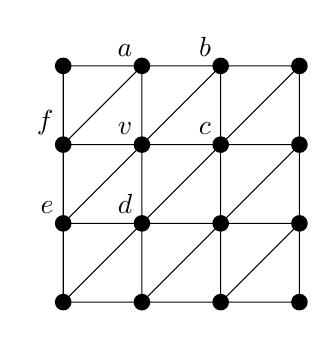
\begin{tikzpicture}
  \draw
    (0, 0) grid[step=1cm] (3, 3)
    (0, 2) -- (1, 3)
    (0, 1) -- (2, 3)
    (0, 0) -- (3, 3)
    (1, 0) -- (3, 2)
    (2, 0) -- (3, 1)
  ;
  \fill[radius=3pt]
    \foreach \x in {0, ..., 3} {
      \foreach \y in {0, ..., 3} {
        (\x, \y) circle[]
      }
    }
  ;
  \path[above left]
    \foreach \p/\v in {
      {1, 3}/a,
      {2, 3}/b,
      {0, 2}/f,
      {1, 2}/v,
      {2, 2}/c,
      {0, 1}/e,
      {1, 1}/d%
    } {
      (\p) node {$\v$}
    }
  ;
\end{tikzpicture}
\caption{The link of \( v \) in this complex consists of the vertices \( \{a,b,c,d,e,f\} \) and the edges \( \{ab,bc,cd,de,ef,fa\} \), forming a hexagon.}
\label{fig:link}
\end{figure}

\begin{mydef}
A \defemph{combinatorial manifold} (or \defemph{combinatorial triangulation}) of dimension \( n \) is a simplicial complex of dimension \( n \) such that the link of every vertex is a simplicial sphere of dimension \( n-1 \) (i.e. its geometric realization is homeomorphic to an \( n-1 \)-sphere). Denote by \( \combmfdset \) the type of combinatorial manifolds of dimension \( n \) (which the notation again reminds us are sets).
\end{mydef}

In a 2-dimensional combinatorial manifold the link is a polygon. See Figures~\ref{fig:sphere_triangulation}, \ref{fig:torus_wiki_triangulation}, and \ref{fig:genus3_wiki_triangulation} for some examples of 2-dimensional combinatorial manifolds of genus 0, 1, and 3.

A classical 1940 result of Whitehead, building on Cairn, states that every smooth manifold admits a combinatorial triangulation\cite{whitehead_triangulation}. So it appears reasonably well motivated to study this class of objects.

\begin{figure}[htbp]
\centering
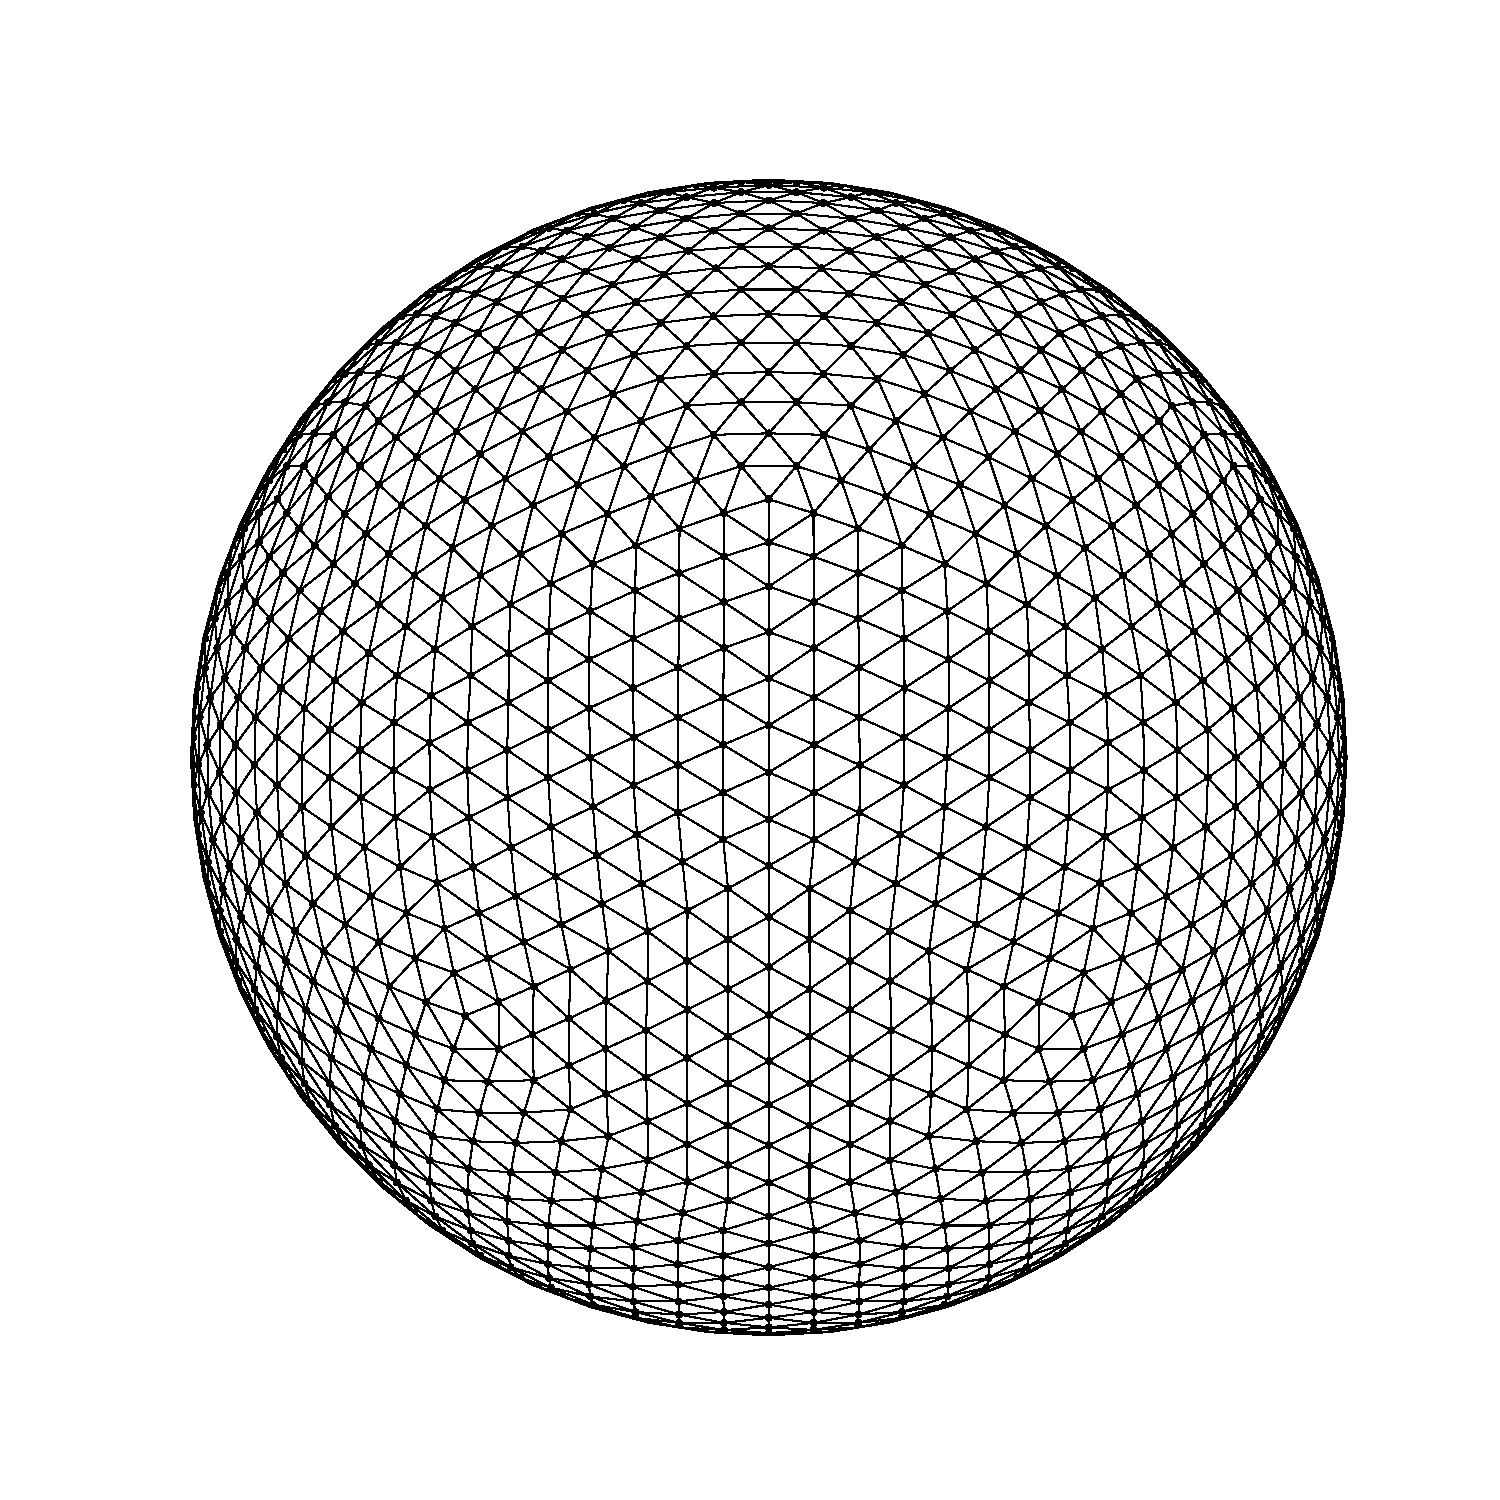
\includegraphics[width=200pt]{triangulated_sphere.pdf}
\caption{A combinatorial triangulation of a sphere, created with stripy.}
\label{fig:sphere_triangulation}
\end{figure}

\begin{figure}[htbp]
\centering
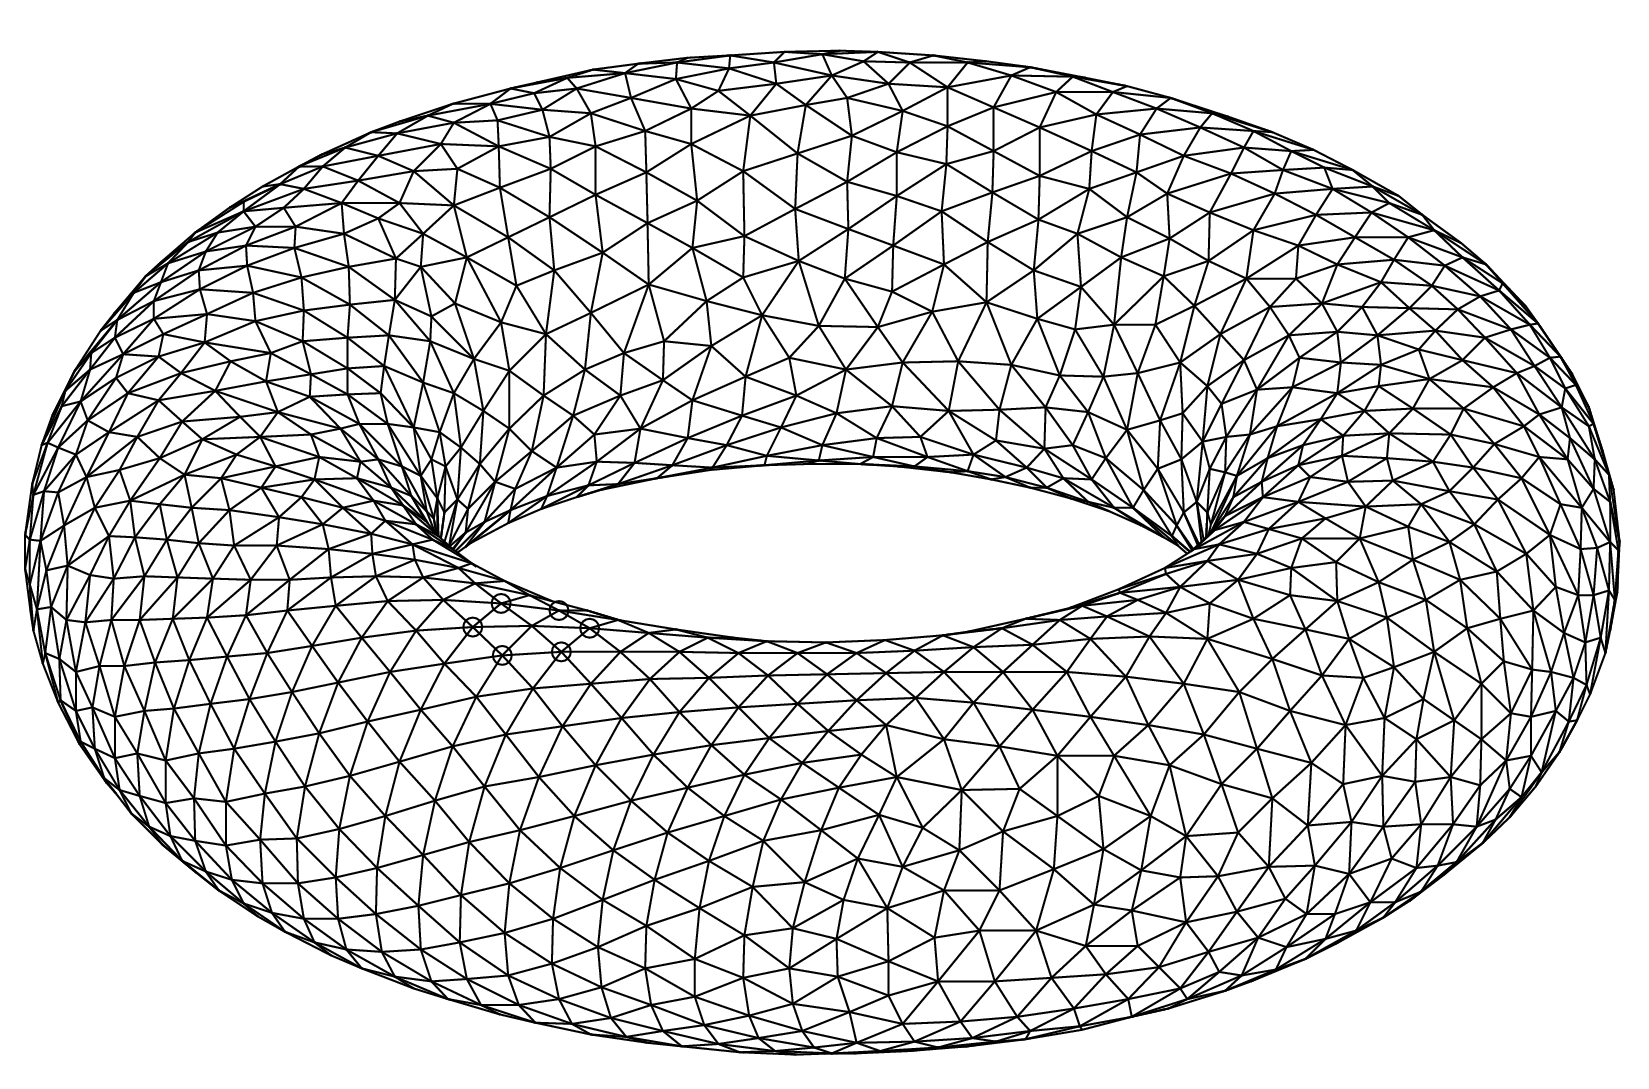
\includegraphics[width=200pt]{Torus-triang.png}
\caption{A torus with an interesting triangulation, from Wikipedia. The links have various vertex counts from 5-7. Clearly a constant value of 6 would also work. (By Ag2gaeh - Own work, CC BY-SA 3.0, https://commons.wikimedia.org/w/index.php?curid=30856793)}
\label{fig:torus_wiki_triangulation}
\end{figure}

\begin{figure}[htbp]
\centering
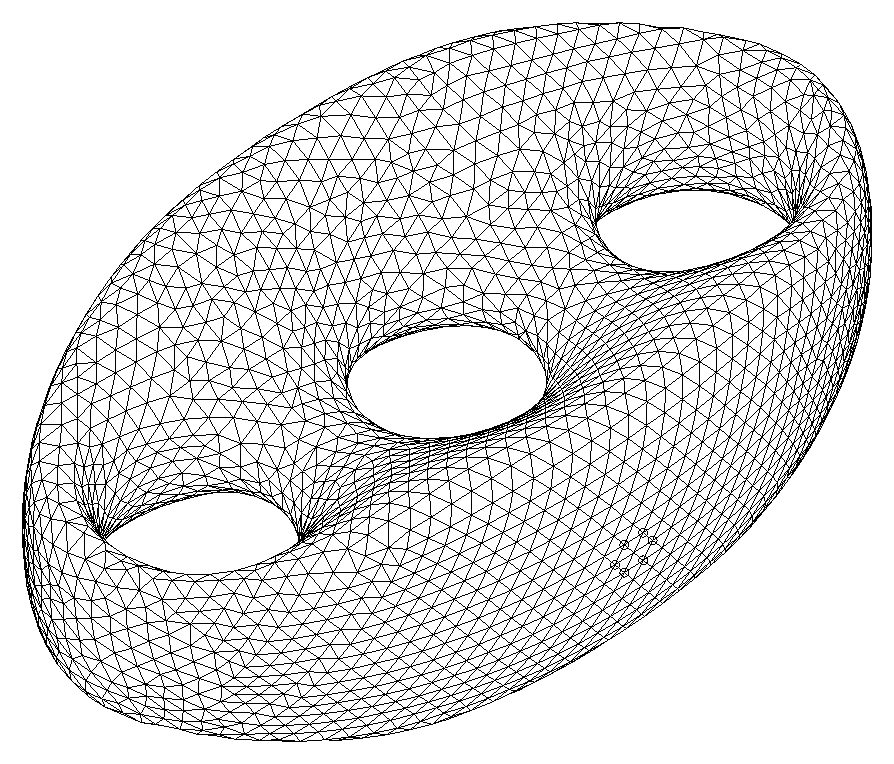
\includegraphics[width=200pt]{triangulated_genus3.pdf}
\caption{A 3-holes torus with triangulation, from Wikipedia. (By Ag2gaeh - Own work, CC BY-SA 3.0, https://commons.wikimedia.org/wiki/File:Tri-brezel.svg)}
\label{fig:genus3_wiki_triangulation}
\end{figure}

\subsection{Higher inductive combinatorial manifolds}

To convert a simplicial complex \( M \) of dimension at most 2 to a higher inductive type, we will convert the data in each classical dimension to a path constructor of the corresponding HoTT dimension.

\begin{mydef}
The function \( \mathcal{R}:\simcompt\to\Type \) is called \defemph{realization} and creates a higher inductive type from the data of a simplicial complex. Given \( M:\simcompt \) then \( \mathcal{R}(M) \) is given by
\begin{enumerate}
\item vertices: a function \( \mathsf{v_0}:M_0\to \mathcal{R}(M) \) serving as the 0-dimensional constructors
\item edges: a function \( \mathsf{v_1} \) on 1-faces, sending \( \{a, b\}\mapsto \mathsf{v_0}(a)=\mathsf{v_0}(b) \)
\item 2-faces: a function \( \mathsf{v_2} \) on 2-faces, sending \( \{a, b, c\}\mapsto \refl_a = \mathsf{v_1}(\{a, b\})\cdot \mathsf{v_1}(\{b, c\})\cdot \mathsf{v_1}(\{a, c\})^{-1} \).
\end{enumerate}
\end{mydef}

\subsection{Polygons}\label{sec:polygons}

We will begin with a type that is important both for the domain and the codomain of mere circles: a square.

\begin{mydef}
The higher inductive type \( C_4 \) (where C stands for ``circle'').
\begin{align*}
C_4 &: \Type \\
c_1, c_2, c_3, c_4 &: C_4 \\
c_1c_2 &: c_1 = c_2 \\
c_2c_3 &: c_2 = c_3 \\
c_3c_4 &: c_3 = c_4 \\
c_4c_1 &: c_4 = c_1 \\
\end{align*}
\end{mydef}

\begin{figure}[htbp]
\centering
\begin{tikzpicture}[
node distance = 15mm and 15mm,
V/.style = {circle, fill, draw=black, inner sep=1pt, font=\footnotesize},
every edge quotes/.style = {auto, font=\footnotesize},
arrow/.style={->,semithick}
]
\begin{scope}[nodes=V]
  \node[label=above left:\( c_1 \)] (1) {};
  \node[label=above right:\( c_2 \)] (2) [right=of 1]  {};
  \node[label=below right:\( c_3 \)] (3) [below=of 2]  {};
  \node[label=below left:\( c_4 \)] (4) [below=of 1]  {};
\end{scope}
\draw[arrow]
        (1)  edge["\( c_1c_2 \)"] (2)
        (2)  edge["\( c_2c_3 \)"] (3)
        (3)  edge["\( c_3c_4 \)"] (4)
        (4)  edge["\( c_4c_1 \)"] (1);
\end{tikzpicture}

\caption{The HIT \( C_4 \).}
\end{figure}

The standard HoTT circle itself is a non-example of a combinatorial manifold since it lacks the second vertex of the edge:

\begin{mydef}
The higher inductive type \( \so \):
\begin{align*}
\so &:\Type \\
\mathsf{base}&:\so \\
\mathsf{loop}&:\mathsf{base}=\mathsf{base}
\end{align*}
\end{mydef}

Nonetheless, all polygons are equivalent to each other and to \( \so \).

\begin{mylemma}
The function \( \ell:C_4\to\so \) given by \( \ell(c_i)=\mathsf{base} \) for all \( i \), and \( \ell(c_ic_j)=\mathsf{loop} \) for all \( i,j \) is an equivalence with inverse \( \ell^{-1}(\mathsf{base})=c_1 \) and \( \ell^{-1}(\mathsf{loop})=c_1c_2\cdot c_2c_3\cdot c_3c_4\cdot c_4c_1 \). There are clearly other inverses for different choices of vertex.
\end{mylemma}
\begin{proof}
We can adapt the proof in the HoTT Book\cite{hottbook} of Lemma 6.5.1 which proves that \( \Sigma\mathbf{2}\simeq S^1 \).
\end{proof}

Recalling that terms of \( \EMzo \) are pairs: a type, and a mere equivalence with \( \so \), we have:

\begin{mycor}
We have \( (C_4,||\ell||_{-1}):\EMzo. \)
\end{mycor}

Real-world triangulations of surfaces will often have links whose number of vertices varies across the surface. For example we can see hexagons and pentagons in Figure~\ref{fig:sphere_triangulation}. This presumably introduces only a minor practical inconvenience and doesn't materially affect the discussion to come.

\subsection{\texorpdfstring{The higher inductive type \( \oo \)}{The higher inductive type O}}

We will create our first combinatorial surface, a 2-sphere. We will adopt the convention that a subscript indicates the dimension of a subskeleton of a complex. For instance, we have \( \mathsf{base}:\so_0 \).

\begin{mydef}
The HIT \( \oo_0 \) is just 6 points, intended as the 0-skeleton of an octahedron, with vertices named after the colors on the faces of a famous Central European puzzle cube.
\[ w, y, b, r, g, o : \oo_0 \]
\end{mydef}

\begin{mydef}
The HIT \( \oo_1 \) is the 1-skeleton of an octahedron.
\begin{align*}
w, y, b, r, g, o &: \oo_1 & yg &: y=g \\
wb &: w=b & yo &: y=o \\
wr &: w=r & br &: b=r \\
wg &: w=g & rg &: r=g \\
wo &: w=o & go &: g=o \\
yb &: y=b & ob &: o=b \\
yr &: y=r
\end{align*}
\end{mydef}

\begin{mydef}
The HIT \( \oo \) is an octahedron:
\begin{align*}
w, y, b, r, g, o &: \oo \\
wb &: w=b & br &: b=r & wbr &: wb\cdot br\cdot wr^{-1} = \refl_w \\
wr &: w=r & rg &: r=g & wrg &: wr\cdot rg\cdot wg^{-1} = \refl_w \\
wg &: w=g & go &: g=o & wgo &: wg\cdot go\cdot wo^{-1} = \refl_w \\
wo &: w=o & ob &: o=b & wob &: wo\cdot ob\cdot wb^{-1} = \refl_w \\
yb &: y=b & & & yrb &: yr\cdot rb\cdot yb^{-1} = \refl_y \\
yr &: y=r & & & ygr &: yg\cdot gr\cdot yr^{-1} = \refl_y \\
yg &: y=g & & & yog &: yo\cdot og\cdot yg^{-1} = \refl_y \\
yo &: y=o & & & ybo &: yb\cdot bo\cdot yo^{-1} = \refl_y 
\end{align*}
\end{mydef}

\begin{figure}[htbp]
\centering
\begin{figure}[h]
\centering
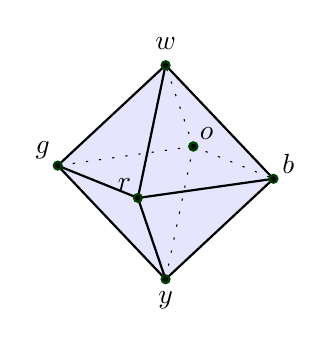
\begin{tikzpicture}%
  [x={(-0.860769cm, -0.121512cm)},
  y={(0.508996cm, -0.205391cm)},
  z={(-0.000053cm, 0.971107cm)},
  scale=1,
  back/.style={loosely dotted, thin},
  edge/.style={black, thick},
  facet/.style={fill=blue!95!black,fill opacity=0.1},
  vertex/.style={inner sep=1pt,circle,draw=green!25!black,fill=black,thick}]
\coordinate (-1, -1, 0) at (-1, -1, 0);
\coordinate (-1, 1, 0) at (-1, 1, 0);
\coordinate (0, 0, -1) at (0, 0, -1);
\coordinate (0, 0, 1) at (0, 0, 1);
\coordinate (1, -1, 0) at (1, -1, 0);
\coordinate (1, 1, 0) at (1, 1, 0);
%% Drawing edges in the back
%%
\draw[edge,back] (-1, -1, 0) -- (-1, 1, 0);
\draw[edge,back] (-1, -1, 0) -- (0, 0, -1.4);
\draw[edge,back] (-1, -1, 0) -- (0, 0, 1.4);
\draw[edge,back] (-1, -1, 0) -- (1, -1, 0);
%% Drawing vertices in the back
%%
\node[vertex] at (-1, -1, 0)     {};
%% Drawing the facets
%%
\fill[facet] (1, 1, 0) -- (0, 0, -1.4) -- (1, -1, 0) -- cycle {};
\fill[facet] (1, 1, 0) -- (0, 0, 1.4) -- (1, -1, 0) -- cycle {};
\fill[facet] (1, 1, 0) -- (-1, 1, 0) -- (0, 0, 1.4) -- cycle {};
\fill[facet] (1, 1, 0) -- (-1, 1, 0) -- (0, 0, -1.4) -- cycle {};
%% Drawing edges in the front
%%
\draw[edge] (-1, 1, 0) -- (0, 0, -1.4);
\draw[edge] (-1, 1, 0) -- (0, 0, 1.4);
\draw[edge] (-1, 1, 0) -- (1, 1, 0);
\draw[edge] (0, 0, -1.4) -- (1, -1, 0);
\draw[edge] (0, 0, -1.4) -- (1, 1, 0);
\draw[edge] (0, 0, 1.4) -- (1, -1, 0);
\draw[edge] (0, 0, 1.4) -- (1, 1, 0);
\draw[edge] (1, -1, 0) -- (1, 1, 0);
%% Drawing the vertices in the front
%%
\begin{scope}[nodes=vertex]
\node[label=above right:\( b \)] at (-1, 1, 0)     {};
\node[label=below:\( y \)] at (0, 0, -1.4)     {};
\node[label=above:\( w \)] at (0, 0, 1.4)     {};
\node[label=above left:\( g \)] at (1, -1, 0)     {};
\node[label=above left:\( r \)] at (1, 1, 0)     {};
\node[label=above right:\( o \)] at (-1, -1, 0)     {};
\end{scope}
\end{tikzpicture}
\caption{The HIT \( \oo \) which has 6 points, 12 1-paths, 8 2-paths.}
\end{figure}

\caption{The HIT \( \oo \) which has 6 points, 12 1-paths, 8 2-paths.}
\end{figure}

We have obvious maps \( \oo_0\xrightarrow[]{i_0} \oo_1\xrightarrow[]{i_1} \oo \) that include each skeleton into the next-higher-dimensional skeleton.

\subsection{Groupoid operations on higher inductive combinatorial manifolds}

Let \( M:\simcompt \) be a combinatorial 2-manifold and \( \mm\defeq\mathcal{R}(M):\combmfdt \) its realization as a higher inductive type. \( \mm \) has triangular 2-faces just as \( M \) does, except they are 2-paths in the HoTT sense. If two faces \( bca \) and \( bdc \) share the edge \( bc \) (see Figure~\ref{fig:concat}), then we can form the type \( bca':ba\cdot ac = bc \) by reorganizing the face as a path from the concatenation of two edges to the third edge. Similarly we can form \( bdc':bd\cdot dc=bc \). We can now concatenate these:
\[ 
bca'\cdot bdc'^{-1}: ba\cdot ac = bd\cdot dc
\] 
which fills the 4-gon \( abdc \), and so can be reorganized as a path \( abdc:\refl_a=\refl_a \) or a path \( bdca:\refl_b=\refl_b \) or other possibilities.
\begin{figure}[htbp]
\centering
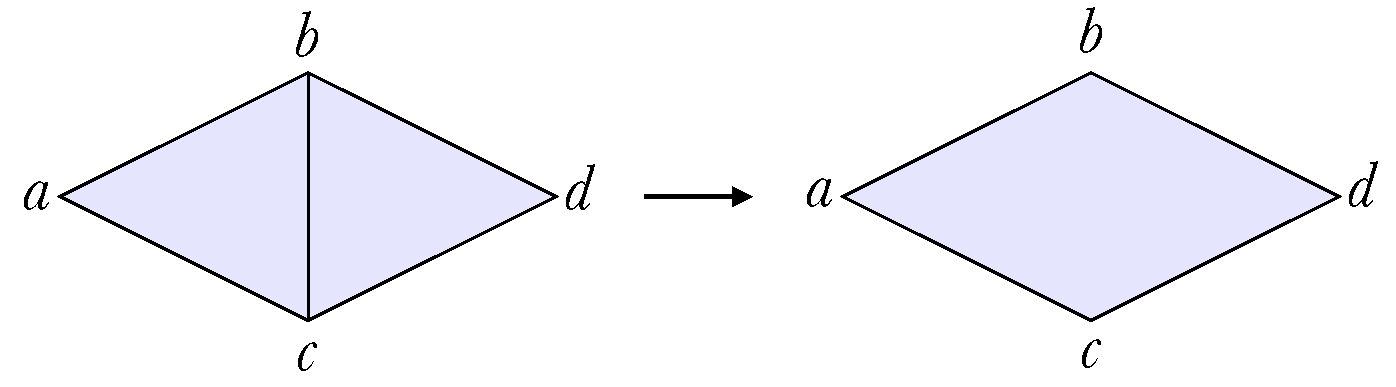
\includegraphics[width=200pt]{concat.pdf}
\caption{Concatenating the triangles \( abc \) and \( bdc \) gives the 4-gon \( abdc \).}
\label{fig:concat}
\end{figure}

We will have two use cases for this operation. The first is to consider the concatenation of \emph{all} the faces of \( \mm \), which if we choose a base point \( x:\mm \) is a path from \( \refl_x \) to itself. This will play the role of the ``fundamental homology class'' from classical topology, which is an object on which 2-forms can be evaluated to compute their value on the whole manifold. 

\begin{mydef}
\label{def:totalface}
If \( \mm:\combmfdt \) is a combinatorial manifold and \( v:\mm_0 \) is a vertex, a \( total face \) of \( \mm \) is any concatenation of all the data in \( \mm \) that produces a term in \( \refl_v=\refl_v \).
\end{mydef}

The second use case for concatenating faces is to create an \emph{equivalent} type to \( \mm \) but without one of the point constructors. Figure~\ref{fig:hex_concat} illustrates the equivalence.
\begin{figure}[htbp]
\centering
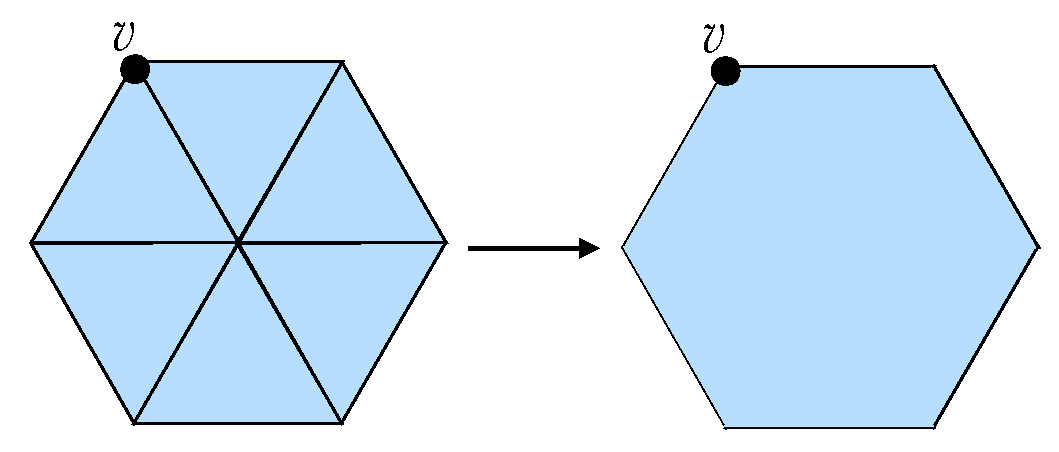
\includegraphics[width=200pt]{hex_concat.pdf}
\caption{Concatenating the six triangles in the approrpiate way produces a 2-path in \( \refl_v=\refl_v \).}
\label{fig:hex_concat}
\end{figure}

\begin{mydef}
If \( \mm:\combmfdt \) is a combinatorial manifold and \( Z\subset \mm_0 \) is a set of vertices in \( \mm \) with members \( Z=\{z_0,\ldots,z_n\} \), then denote by \( \mm\setminus Z \) the type given by omitting the vertices in \( Z \) from the constructors in all dimensions where they appeared. Call the points of \( Z \) \defemph{isolated} if no two of them are neighbors, i.e. we have \( \pit{z:Z}\link(z)\cap Z=\emptyset \). In the isolated case \( \mm\setminus Z \) has boundary circles where each vertex was removed.
\end{mydef}

\begin{mydef}
\label{def:replacement}
If we have \( \mm\setminus Z \) for some isolated set of verticies \( Z \), then for each \( z:Z \) we can compose all the faces which contain \( z \), forming a new face (see Figure~\ref{fig:hex_concat}). In this way we produce an equivalent type \( \mm_Z\simeq \mm \) but which is no longer combinatorial since we have erased some of the edges from some of the neighborhoods. We call \( \mm_Z \) the \defemph{replacement of \( \mm \) without \( Z \)}.
\end{mydef}

\subsection{The function \texorpdfstring{\( \link \)}{link}}

Taking the link of a vertex gives us a map to polygons.

\begin{mydef}
\( \link:\oo_0\to\EMzo \) is given by:
\begin{align*}
\link(w) &= brgo & \link(r) &= wbyg \\
\link(y) &= bogr & \link(g) &= wryo \\
\link(b) &= woyr & \link(o) &= wgyb
\end{align*}
We chose these orderings for the vertices in the link, by visualizing standing at the given vertex as if it were the north pole, then looking south and enumerating the link in clockwise order, starting from \( w \) if possible, else \( b \).
\end{mydef}

\begin{figure}[htbp]
\centering
\begin{figure}[h]
\centering
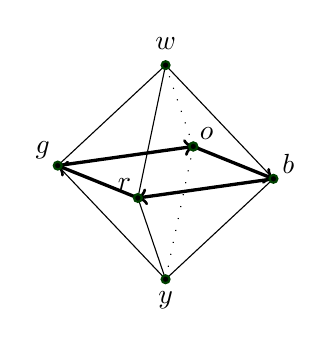
\begin{tikzpicture}%
  [x={(-0.860769cm, -0.121512cm)},
  y={(0.508996cm, -0.205391cm)},
  z={(-0.000053cm, 0.971107cm)},
  scale=1,
  eqback/.style={->, very thick},
  back/.style={loosely dotted, thin},
  eqedge/.style={->, very thick},
  edge/.style={black, thin},
  facet/.style={fill=blue!95!black,fill opacity=0.0},
  vertex/.style={inner sep=1pt,circle,draw=green!25!black,fill=black,thick}]
\coordinate (-1, -1, 0) at (-1, -1, 0);
\coordinate (-1, 1, 0) at (-1, 1, 0);
\coordinate (0, 0, -1) at (0, 0, -1);
\coordinate (0, 0, 1) at (0, 0, 1);
\coordinate (1, -1, 0) at (1, -1, 0);
\coordinate (1, 1, 0) at (1, 1, 0);
%% Drawing edges in the back
%%
\draw[edge,eqback] (-1, -1, 0) -- (-1, 1, 0);
\draw[edge,back] (-1, -1, 0) -- (0, 0, -1.4);
\draw[edge,back] (-1, -1, 0) -- (0, 0, 1.4);
\draw[edge,eqback] (1, -1, 0) -- (-1, -1, 0);
%% Drawing vertices in the back
%%
\node[vertex] at (-1, -1, 0)     {};
%% Drawing the facets
%%
\fill[facet] (1, 1, 0) -- (0, 0, -1.4) -- (1, -1, 0) -- cycle {};
\fill[facet] (1, 1, 0) -- (0, 0, 1.4) -- (1, -1, 0) -- cycle {};
\fill[facet] (1, 1, 0) -- (-1, 1, 0) -- (0, 0, 1.4) -- cycle {};
\fill[facet] (1, 1, 0) -- (-1, 1, 0) -- (0, 0, -1.4) -- cycle {};
%% Drawing edges in the front
%%
\draw[edge] (-1, 1, 0) -- (0, 0, -1.4);
\draw[edge] (-1, 1, 0) -- (0, 0, 1.4);
\draw[eqedge] (-1, 1, 0) -- (1, 1, 0);
\draw[edge] (0, 0, -1.4) -- (1, -1, 0);
\draw[edge] (0, 0, -1.4) -- (1, 1, 0);
\draw[edge] (0, 0, 1.4) -- (1, -1, 0);
\draw[edge] (0, 0, 1.4) -- (1, 1, 0);
\draw[eqedge] (1, 1, 0) -- (1, -1, 0);
%% Drawing the vertices in the front
%%
\begin{scope}[nodes=vertex]
\node[label=above right:\( b \)] at (-1, 1, 0)     {};
\node[label=below:\( y \)] at (0, 0, -1.4)     {};
\node[label=above:\( w \)] at (0, 0, 1.4)     {};
\node[label=above left:\( g \)] at (1, -1, 0)     {};
\node[label=above left:\( r \)] at (1, 1, 0)     {};
\node[label=above right:\( o \)] at (-1, -1, 0)     {};
\end{scope}
\end{tikzpicture}

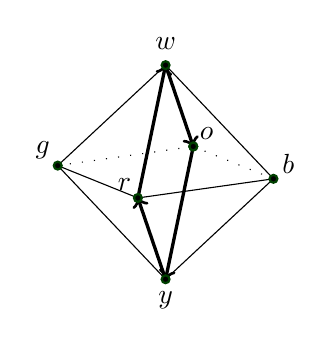
\begin{tikzpicture}%
  [x={(-0.860769cm, -0.121512cm)},
  y={(0.508996cm, -0.205391cm)},
  z={(-0.000053cm, 0.971107cm)},
  scale=1,
  eqback/.style={->, very thick},
  back/.style={loosely dotted, thin},
  eqedge/.style={->, very thick},
  edge/.style={black, thin},
  facet/.style={fill=blue!95!black,fill opacity=0.0},
  vertex/.style={inner sep=1pt,circle,draw=green!25!black,fill=black,thick}]
\coordinate (-1, -1, 0) at (-1, -1, 0);
\coordinate (-1, 1, 0) at (-1, 1, 0);
\coordinate (0, 0, -1) at (0, 0, -1);
\coordinate (0, 0, 1) at (0, 0, 1);
\coordinate (1, -1, 0) at (1, -1, 0);
\coordinate (1, 1, 0) at (1, 1, 0);
%% Drawing edges in the back
%%
\draw[edge,back] (-1, -1, 0) -- (-1, 1, 0);
\draw[edge,eqback] (-1, -1, 0) -- (0, 0, -1.4);
\draw[edge,eqback] (0, 0, 1.4) -- (-1, -1, 0);
\draw[edge,back] (1, -1, 0) -- (-1, -1, 0);
%% Drawing vertices in the back
%%
\node[vertex] at (-1, -1, 0)     {};
%% Drawing the facets
%%
\fill[facet] (1, 1, 0) -- (0, 0, -1.4) -- (1, -1, 0) -- cycle {};
\fill[facet] (1, 1, 0) -- (0, 0, 1.4) -- (1, -1, 0) -- cycle {};
\fill[facet] (1, 1, 0) -- (-1, 1, 0) -- (0, 0, 1.4) -- cycle {};
\fill[facet] (1, 1, 0) -- (-1, 1, 0) -- (0, 0, -1.4) -- cycle {};
%% Drawing edges in the front
%%
\draw[edge] (-1, 1, 0) -- (0, 0, -1.4);
\draw[edge] (-1, 1, 0) -- (0, 0, 1.4);
\draw[edge] (-1, 1, 0) -- (1, 1, 0);
\draw[edge] (0, 0, -1.4) -- (1, -1, 0);
\draw[eqedge] (0, 0, -1.4) -- (1, 1, 0);
\draw[edge] (0, 0, 1.4) -- (1, -1, 0);
\draw[eqedge] (1, 1, 0) -- (0, 0, 1.4) ;
\draw[edge] (1, 1, 0) -- (1, -1, 0);
%% Drawing the vertices in the front
%%
\begin{scope}[nodes=vertex]
\node[label=above right:\( b \)] at (-1, 1, 0)     {};
\node[label=below:\( y \)] at (0, 0, -1.4)     {};
\node[label=above:\( w \)] at (0, 0, 1.4)     {};
\node[label=above left:\( g \)] at (1, -1, 0)     {};
\node[label=above left:\( r \)] at (1, 1, 0)     {};
\node[label=above right:\( o \)] at (-1, -1, 0)     {};
\end{scope}
\end{tikzpicture}

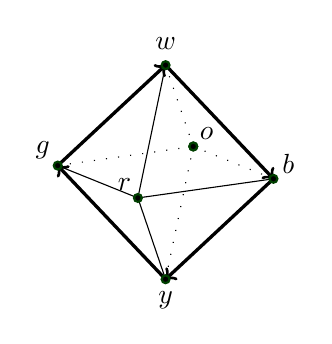
\begin{tikzpicture}%
  [x={(-0.860769cm, -0.121512cm)},
  y={(0.508996cm, -0.205391cm)},
  z={(-0.000053cm, 0.971107cm)},
  scale=1,
  eqback/.style={->, very thick},
  back/.style={loosely dotted, thin},
  eqedge/.style={->, very thick},
  edge/.style={black, thin},
  facet/.style={fill=blue!95!black,fill opacity=0.0},
  vertex/.style={inner sep=1pt,circle,draw=green!25!black,fill=black,thick}]
\coordinate (-1, -1, 0) at (-1, -1, 0);
\coordinate (-1, 1, 0) at (-1, 1, 0);
\coordinate (0, 0, -1) at (0, 0, -1);
\coordinate (0, 0, 1) at (0, 0, 1);
\coordinate (1, -1, 0) at (1, -1, 0);
\coordinate (1, 1, 0) at (1, 1, 0);
%% Drawing edges in the back
%%
\draw[edge,back] (-1, -1, 0) -- (-1, 1, 0);
\draw[edge,back] (-1, -1, 0) -- (0, 0, -1.4);
\draw[edge,back] (-1, -1, 0) -- (0, 0, 1.4);
\draw[edge,back] (1, -1, 0) -- (-1, -1, 0);
%% Drawing vertices in the back
%%
\node[vertex] at (-1, -1, 0)     {};
%% Drawing the facets
%%
\fill[facet] (1, 1, 0) -- (0, 0, -1.4) -- (1, -1, 0) -- cycle {};
\fill[facet] (1, 1, 0) -- (0, 0, 1.4) -- (1, -1, 0) -- cycle {};
\fill[facet] (1, 1, 0) -- (-1, 1, 0) -- (0, 0, 1.4) -- cycle {};
\fill[facet] (1, 1, 0) -- (-1, 1, 0) -- (0, 0, -1.4) -- cycle {};
%% Drawing edges in the front
%%
\draw[eqedge] (-1, 1, 0) -- (0, 0, -1.4);
\draw[eqedge] (0, 0, 1.4) -- (-1, 1, 0);
\draw[edge] (-1, 1, 0) -- (1, 1, 0);
\draw[eqedge] (0, 0, -1.4) -- (1, -1, 0);
\draw[edge] (0, 0, -1.4) -- (1, 1, 0);
\draw[eqedge] (1, -1, 0) -- (0, 0, 1.4);
\draw[edge] (0, 0, 1.4) -- (1, 1, 0);
\draw[edge] (1, 1, 0) -- (1, -1, 0);
%% Drawing the vertices in the front
%%
\begin{scope}[nodes=vertex]
\node[label=above right:\( b \)] at (-1, 1, 0)     {};
\node[label=below:\( y \)] at (0, 0, -1.4)     {};
\node[label=above:\( w \)] at (0, 0, 1.4)     {};
\node[label=above left:\( g \)] at (1, -1, 0)     {};
\node[label=above left:\( r \)] at (1, 1, 0)     {};
\node[label=above right:\( o \)] at (-1, -1, 0)     {};
\end{scope}
\end{tikzpicture}
\caption{The equators for \( w, b, r \).}
\end{figure}
\caption{\( \link \) for the verticies \( w, b\) and \( r \).}
\label{fig:triangle_of_equators}
\end{figure}

To extend \( \link \) to the 1-skeleton we have complete freedom. We will do something ``tangent bundley'', imagining how \( \link \) changes as we slide from point to point in the embedding shown in the figures. Sliding from \( w \) to \( b \) and tipping the link as we go, we see \( r\mapsto r \) and \( o\mapsto o \) because those lie on the axis of rotation. Then \( g\mapsto w \) and \( b\mapsto y \). 

\begin{mydef}
Define \( T_1:\oo_1\to\EMzo \) on just the 1-skeleton by extending \( \link \) as follows:
Transport away from \( w \):
\begin{itemize}
\item \( T_1(wb):[b, r, g, o]\mapsto [y, r, w, o] \) (\( r, o \) fixed)
\item \( T_1(wr):[b, r, g, o]\mapsto [b, y, g, w] \) (\( b, g \) fixed)
\item \( T_1(wg):[b, r, g, o]\mapsto [w, r, y, o] \)
\item \( T_1(wo):[b, r, g, o]\mapsto [b, w, g, y] \)
\end{itemize}
Transport away from \( y \):
\begin{itemize}
\item \( T_1(yb):[b, o, g, r]\mapsto [w, o, y, r] \)
\item \( T_1(yr):[b, o, g, r]\mapsto [b, y, g, w] \)
\item \( T_1(yg):[b, o, g, r]\mapsto [y, o, w, r] \)
\item \( T_1(yo):[b, o, g, r]\mapsto [b, w, g, y] \)
\end{itemize}
Transport along the equator:
\begin{itemize}
\item \( T_1(br):[w, o, y, r]\mapsto [w, b, y, g] \) 
\item \( T_1(rg):[w, b, y, g]\mapsto [w, r, y, o] \)
\item \( T_1(go):[w, r, y, o]\mapsto [w, g, y, b] \)
\item \( T_1(ob):[w, g, y, b]\mapsto [w, o, y, r] \)
\end{itemize}
\end{mydef}

It's very important to be able to visualize what \( T_1 \) does to triangular paths such as \( wb\cdot br\cdot rw \) (which circulates around the boundary of face \( wbr \)). You can see it if you imagine Figure~\ref{fig:triangle_of_equators} as the frames of a short movie. Or you can place your palm over the top of a cube and note where your fingers are pointing, then slide your hand to an equatorial face, then along the equator, then back to the top. The answer is: you come back rotated clockwise by a quarter-turn. 

\begin{mydef}
The map \( R:C_4\to C_4 \) rotates by one quarter turn, one ``click":
\begin{multicols}{2}
\begin{itemize}
\item \( R(c_1) = c_2 \)
\item \( R(c_2) = c_3 \)
\item \( R(c_3) = c_4 \)
\item \( R(c_4) = c_1 \)
\item \( R(c_1c_2) = c_2c_3 \)
\item \( R(c_2c_3) = c_3c_4 \)
\item \( R(c_3c_4) = c_4c_1 \)
\item \( R(c_4c_1) = c_1c_2 \)
\end{itemize}
\end{multicols}
\end{mydef}

Now let's extend \( T_1 \) to all of \( \oo \) by providing values for the eight faces. The face \( wbr \) is a path from \( \refl_w \) to the concatenation \( wb\cdot br\cdot rw \), and so the image of \( wbr \) under the extended version of \( T_1 \) must be a homotopy from \( \refl_{T_1(w)} \) to \( T_1(wb\cdot br\cdot rw) \). Here there is no additional freedom.

\begin{mydef}
Define \( T_2:\oo\to\EMzo \) by extending \( T_1 \) to the faces as follows:
\begin{multicols}{2}
\begin{itemize}
\item \( T_2(wbr)=H_R \) 
\item \( T_2(wrg)=H_R \)
\item \( T_2(wgo)=H_R \)
\item \( T_2(ybo)=H_R \)
\item \( T_2(yrb)=H_R \) 
\item \( T_2(ygr)=H_R \)
\item \( T_2(yog)=H_R \)
\item \( T_2(ybo)=H_R \)
\end{itemize}
\end{multicols}
where \( H_R:R=\refl \) is the obvious homotopy.
\end{mydef}

All the faces do the same thing: they map to a homotopy between the identity and clockwise rotation by a quarter turn. Concatenating the eight faces in the 2-groupoid \( \oo \) would then map to a homotopy between the identity and two full rotations. This makes visible in HoTT the link between curvature and the Euler characteristic (which is 2 for the octahedron). More on that later.

\subsection{The torus}

We can define a combinatorial torus as a similar HIT. This time each vertex will have six neighbors. So all the links will be merely equal to \( C_6 \) which is a hexagonal version of \( C_4 \). See Figure~\ref{fig:torus}. 

To help parse this figure, imagine instead Figure~\ref{fig:flattorus}. We take this simple alternating-triangle pattern, then glue the left and right edges, then bend into Figure~\ref{fig:torus}. The fact that each column in Figure~\ref{fig:flattorus} has four dots corresponds to the torus in Figure~\ref{fig:torus} having a square in front, diamonds in the middle, and a square in back.

\begin{figure}[htbp]
\centering
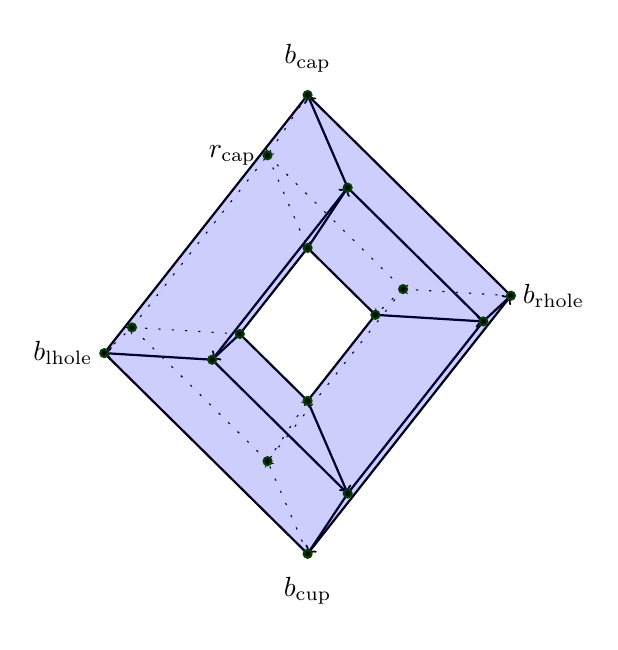
\begin{tikzpicture}%
  [x={(-0.860769cm, -0.121512cm)},
  y={(0.508996cm, -0.205391cm)},
  z={(-0.000053cm, 0.971107cm)},
  scale=1,
  back/.style={loosely dotted, thin},
  edge/.style={->,black, thick},
  line/.style={black, thick},
  facet/.style={fill=blue!95!black,fill opacity=0.1},
  vertex/.style={inner sep=1pt,circle,draw=green!25!black,fill=black,thick}]
\coordinate (r_cap) at (0, -1, 5);
\coordinate (g_cap) at (0, 0, 4 );
\coordinate (o_cap) at (0, 1, 5 );
\coordinate (b_cap) at (0, 0, 6 );

\coordinate (r_cup) at (0, -1, 1);
\coordinate (g_cup) at (0, 0, 2 );
\coordinate (o_cup) at (0, 1, 1 );
\coordinate (b_cup) at (0, 0, 0 );

\coordinate (r_ohole) at (-2, -1, 3);
\coordinate (g_ohole) at (-1, 0,  3);
\coordinate (o_ohole) at (-2, 1,  3);
\coordinate (b_ohole) at (-3, 0,  3);

\coordinate (r_rhole) at (2, -1, 3);
\coordinate (g_rhole) at (1, 0,  3);
\coordinate (o_rhole) at (2, 1,  3);
\coordinate (b_rhole) at (3, 0,  3);

\draw[edge,back] (r_cap) -- (g_cap);
\draw[edge]      (g_cap) -- (o_cap);
\draw[edge]      (o_cap) -- (b_cap);
\draw[edge,back] (b_cap) -- (r_cap);

\draw[edge,back] (r_cup) -- (g_cup);
\draw[edge]      (g_cup) -- (o_cup);
\draw[edge]      (o_cup) -- (b_cup);
\draw[edge,back] (b_cup) -- (r_cup);

\draw[edge,back] (r_ohole) -- (g_ohole);
\draw[edge]      (g_ohole) -- (o_ohole);
\draw[edge]      (o_ohole) -- (b_ohole);
\draw[edge,back] (b_ohole) -- (r_ohole);

\draw[edge,back] (r_rhole) -- (g_rhole);
\draw[edge]      (g_rhole) -- (o_rhole);
\draw[edge]      (o_rhole) -- (b_rhole);
\draw[edge,back] (b_rhole) -- (r_rhole);

\draw[line,back] (r_cap) --   (r_ohole);
\draw[line,back] (r_ohole) -- (r_cup);
\draw[line,back] (r_cup) --   (r_rhole);
\draw[line,back] (r_rhole) -- (r_cap);

\draw[line] (g_cap) --   (g_ohole);
\draw[line] (g_ohole) -- (g_cup);
\draw[line] (g_cup) --   (g_rhole);
\draw[line] (g_rhole) -- (g_cap);

\draw[line] (o_cap) --   (o_ohole);
\draw[line] (o_ohole) -- (o_cup);
\draw[line] (o_cup) --   (o_rhole);
\draw[line] (o_rhole) -- (o_cap);

\draw[line] (b_cap) --   (b_ohole);
\draw[line] (b_ohole) -- (b_cup);
\draw[line] (b_cup) --   (b_rhole);
\draw[line] (b_rhole) -- (b_cap);

\fill[facet] (r_cap) -- (r_ohole) -- (g_ohole) -- (g_cap) -- cycle {};
\fill[facet] (r_cap) -- (r_rhole) -- (g_rhole) -- (g_cap) -- cycle {};
\fill[facet] (r_cap) -- (r_ohole) -- (b_ohole) -- (b_cap) -- cycle {};
\fill[facet] (r_cap) -- (r_rhole) -- (b_rhole) -- (b_cap) -- cycle {};

\fill[facet] (o_cap) -- (o_ohole) -- (g_ohole) -- (g_cap) -- cycle {};
\fill[facet] (o_cap) -- (o_rhole) -- (g_rhole) -- (g_cap) -- cycle {};
\fill[facet] (o_cap) -- (o_ohole) -- (b_ohole) -- (b_cap) -- cycle {};
\fill[facet] (o_cap) -- (o_rhole) -- (b_rhole) -- (b_cap) -- cycle {};

\fill[facet] (r_cup) -- (r_ohole) -- (g_ohole) -- (g_cup) -- cycle {};
\fill[facet] (r_cup) -- (r_rhole) -- (g_rhole) -- (g_cup) -- cycle {};
\fill[facet] (r_cup) -- (r_ohole) -- (b_ohole) -- (b_cup) -- cycle {};
\fill[facet] (r_cup) -- (r_rhole) -- (b_rhole) -- (b_cup) -- cycle {};

\fill[facet] (o_cup) -- (o_ohole) -- (g_ohole) -- (g_cup) -- cycle {};
\fill[facet] (o_cup) -- (o_rhole) -- (g_rhole) -- (g_cup) -- cycle {};
\fill[facet] (o_cup) -- (o_ohole) -- (b_ohole) -- (b_cup) -- cycle {};
\fill[facet] (o_cup) -- (o_rhole) -- (b_rhole) -- (b_cup) -- cycle {};

\begin{scope}[nodes=vertex]
\node[label=left:\( r_{\mathrm{cap}} \)] at (r_cap) {};
\node at (g_cap) {};
\node at (o_cap) {};
\node[label=above:\( b_{\mathrm{cap}} \)] at (b_cap) {};
\node at (r_cup) {};
\node at (g_cup) {};
\node at (o_cup) {};
\node[label=below:\( b_{\mathrm{cup}} \)] at (b_cup) {};
\node at (r_ohole) {};
\node at (g_ohole) {};
\node at (o_ohole) {};
\node[label=right:\( b_{\mathrm{rhole}} \)] at (b_ohole) {};
\node at (r_rhole) {};
\node at (g_rhole) {};
\node at (o_rhole) {};
\node[label=left:\( b_{\mathrm{lhole}} \)] at (b_rhole) {};
\end{scope}
\end{tikzpicture}

\caption{Torus embedded in 3-dimensional space. If you see color in your rendering then black lines trace four square-shaped paths, red ones connect the front square to the middle diamonds, and blue ones connect the back path to the middle ones.}
\label{fig:torus}
\end{figure}

\begin{figure}[htbp]
\centering
% https://q.uiver.app/#q=WzAsMzYsWzEsNCwiXFxidWxsZXQiXSxbMSw2LCJcXGJ1bGxldCJdLFsyLDcsIlxcYnVsbGV0Il0sWzIsNSwiXFxidWxsZXQiXSxbMiwzLCJcXGJ1bGxldCJdLFsxLDgsIlxcYnVsbGV0Il0sWzEsMiwiXFxidWxsZXQiXSxbMywyLCJcXGJ1bGxldCJdLFszLDQsIlxcYnVsbGV0Il0sWzMsNiwiXFxidWxsZXQiXSxbMyw4LCJcXGJ1bGxldCJdLFsyLDEsIlxcYnVsbGV0Il0sWzQsMSwiXFxidWxsZXQiXSxbNSwyLCJcXGJ1bGxldCJdLFs0LDMsIlxcYnVsbGV0Il0sWzUsNCwiXFxidWxsZXQiXSxbNCw1LCJcXGJ1bGxldCJdLFs1LDYsIlxcYnVsbGV0Il0sWzQsNywiXFxidWxsZXQiXSxbNSw4LCJcXGJ1bGxldCJdLFsyLDAsIlxcbWF0aHJte2JhY2t9Il0sWzQsMCwiXFxtYXRocm17ZnJvbnR9Il0sWzEsMCwiXFxtYXRocm17b3V0ZXJ9Il0sWzMsMCwiXFxtYXRocm17aG9sZX0iXSxbNSwwLCJcXG1hdGhybXtvdXRlcn0iXSxbMSwxMCwiXFxidWxsZXQiXSxbMiw5LCJcXGJ1bGxldCJdLFszLDEwLCJcXGJ1bGxldCJdLFs0LDksIlxcYnVsbGV0Il0sWzUsMTAsIlxcYnVsbGV0Il0sWzAsMiwiXFxtYXRocm17dG9wXFwgb2ZcXCBkaWFtb25kc30iXSxbMCw2LCJcXG1hdGhybXtib3R0b21cXCBvZlxcIGRpYW1vbmRzfSJdLFsxLDEsIlxcICJdLFs1LDEsIlxcICJdLFszLDEsIlxcICJdLFswLDEwLCJcXG1hdGhybXt0b3BcXCBvZlxcIGRpYW1vbmRzfSJdLFs0LDMsIiIsMix7InN0eWxlIjp7ImhlYWQiOnsibmFtZSI6Im5vbmUifX19XSxbMywyLCIiLDIseyJzdHlsZSI6eyJoZWFkIjp7Im5hbWUiOiJub25lIn19fV0sWzAsMSwiIiwyLHsic3R5bGUiOnsiaGVhZCI6eyJuYW1lIjoibm9uZSJ9fX1dLFs0LDAsIiIsMSx7ImNvbG91ciI6WzIzNiw5MSw2MF0sInN0eWxlIjp7ImhlYWQiOnsibmFtZSI6Im5vbmUifX19XSxbMCwzLCIiLDEseyJjb2xvdXIiOlsyMzYsOTEsNjBdLCJzdHlsZSI6eyJoZWFkIjp7Im5hbWUiOiJub25lIn19fV0sWzMsMSwiIiwxLHsiY29sb3VyIjpbMjM2LDkxLDYwXSwic3R5bGUiOnsiaGVhZCI6eyJuYW1lIjoibm9uZSJ9fX1dLFsxLDIsIiIsMSx7ImNvbG91ciI6WzIzNiw5MSw2MF0sInN0eWxlIjp7ImhlYWQiOnsibmFtZSI6Im5vbmUifX19XSxbMiw1LCIiLDEseyJjb2xvdXIiOlsyMzYsOTEsNjBdLCJzdHlsZSI6eyJoZWFkIjp7Im5hbWUiOiJub25lIn19fV0sWzEsNSwiIiwxLHsic3R5bGUiOnsiaGVhZCI6eyJuYW1lIjoibm9uZSJ9fX1dLFs2LDQsIiIsMSx7ImNvbG91ciI6WzIzNiw5MSw2MF0sInN0eWxlIjp7ImhlYWQiOnsibmFtZSI6Im5vbmUifX19XSxbNiwwLCIiLDEseyJzdHlsZSI6eyJoZWFkIjp7Im5hbWUiOiJub25lIn19fV0sWzcsOCwiIiwwLHsic3R5bGUiOnsiaGVhZCI6eyJuYW1lIjoibm9uZSJ9fX1dLFs4LDksIiIsMCx7InN0eWxlIjp7ImhlYWQiOnsibmFtZSI6Im5vbmUifX19XSxbOSwxMCwiIiwwLHsic3R5bGUiOnsiaGVhZCI6eyJuYW1lIjoibm9uZSJ9fX1dLFs3LDQsIiIsMCx7ImNvbG91ciI6WzIzNiw5MSw2MF0sInN0eWxlIjp7ImhlYWQiOnsibmFtZSI6Im5vbmUifX19XSxbNCw4LCIiLDAseyJjb2xvdXIiOlsyMzYsOTEsNjBdLCJzdHlsZSI6eyJoZWFkIjp7Im5hbWUiOiJub25lIn19fV0sWzgsMywiIiwwLHsiY29sb3VyIjpbMjM2LDkxLDYwXSwic3R5bGUiOnsiaGVhZCI6eyJuYW1lIjoibm9uZSJ9fX1dLFszLDksIiIsMCx7ImNvbG91ciI6WzIzNiw5MSw2MF0sInN0eWxlIjp7ImhlYWQiOnsibmFtZSI6Im5vbmUifX19XSxbOSwyLCIiLDAseyJjb2xvdXIiOlsyMzYsOTEsNjBdLCJzdHlsZSI6eyJoZWFkIjp7Im5hbWUiOiJub25lIn19fV0sWzIsMTAsIiIsMCx7ImNvbG91ciI6WzIzNiw5MSw2MF0sInN0eWxlIjp7ImhlYWQiOnsibmFtZSI6Im5vbmUifX19XSxbMTEsNCwiIiwwLHsic3R5bGUiOnsiaGVhZCI6eyJuYW1lIjoibm9uZSJ9fX1dLFsxMSw2LCIiLDAseyJjb2xvdXIiOlsyMzYsOTEsNjBdLCJzdHlsZSI6eyJoZWFkIjp7Im5hbWUiOiJub25lIn19fV0sWzExLDcsIiIsMCx7ImNvbG91ciI6WzIzNiw5MSw2MF0sInN0eWxlIjp7ImhlYWQiOnsibmFtZSI6Im5vbmUifX19XSxbMTksMTcsIiIsMCx7InN0eWxlIjp7ImhlYWQiOnsibmFtZSI6Im5vbmUifX19XSxbMTgsMTYsIiIsMCx7InN0eWxlIjp7ImhlYWQiOnsibmFtZSI6Im5vbmUifX19XSxbMTYsMTQsIiIsMCx7InN0eWxlIjp7ImhlYWQiOnsibmFtZSI6Im5vbmUifX19XSxbMTcsMTUsIiIsMCx7InN0eWxlIjp7ImhlYWQiOnsibmFtZSI6Im5vbmUifX19XSxbMTUsMTMsIiIsMCx7InN0eWxlIjp7ImhlYWQiOnsibmFtZSI6Im5vbmUifX19XSxbMTQsMTIsIiIsMCx7InN0eWxlIjp7ImhlYWQiOnsibmFtZSI6Im5vbmUifX19XSxbMTIsNywiIiwwLHsiY29sb3VyIjpbMSw5NSw2MF0sInN0eWxlIjp7ImhlYWQiOnsibmFtZSI6Im5vbmUifX19XSxbMTIsMTMsIiIsMCx7ImNvbG91ciI6WzEsOTUsNjBdLCJzdHlsZSI6eyJoZWFkIjp7Im5hbWUiOiJub25lIn19fV0sWzEzLDE0LCIiLDAseyJjb2xvdXIiOlsxLDk1LDYwXSwic3R5bGUiOnsiaGVhZCI6eyJuYW1lIjoibm9uZSJ9fX1dLFsxNCw4LCIiLDAseyJjb2xvdXIiOlsxLDk1LDYwXSwic3R5bGUiOnsiaGVhZCI6eyJuYW1lIjoibm9uZSJ9fX1dLFsxNCwxNSwiIiwwLHsiY29sb3VyIjpbMSw5NSw2MF0sInN0eWxlIjp7ImhlYWQiOnsibmFtZSI6Im5vbmUifX19XSxbMTUsMTYsIiIsMCx7ImNvbG91ciI6WzEsOTUsNjBdLCJzdHlsZSI6eyJoZWFkIjp7Im5hbWUiOiJub25lIn19fV0sWzgsMTYsIiIsMCx7ImNvbG91ciI6WzEsOTUsNjBdLCJzdHlsZSI6eyJoZWFkIjp7Im5hbWUiOiJub25lIn19fV0sWzE2LDksIiIsMCx7ImNvbG91ciI6WzEsOTUsNjBdLCJzdHlsZSI6eyJoZWFkIjp7Im5hbWUiOiJub25lIn19fV0sWzE2LDE3LCIiLDAseyJjb2xvdXIiOlsxLDk1LDYwXSwic3R5bGUiOnsiaGVhZCI6eyJuYW1lIjoibm9uZSJ9fX1dLFsxNywxOCwiIiwwLHsiY29sb3VyIjpbMSw5NSw2MF0sInN0eWxlIjp7ImhlYWQiOnsibmFtZSI6Im5vbmUifX19XSxbOSwxOCwiIiwwLHsiY29sb3VyIjpbMSw5NSw2MF0sInN0eWxlIjp7ImhlYWQiOnsibmFtZSI6Im5vbmUifX19XSxbMTgsMTksIiIsMCx7ImNvbG91ciI6WzEsOTUsNjBdLCJzdHlsZSI6eyJoZWFkIjp7Im5hbWUiOiJub25lIn19fV0sWzE4LDEwLCIiLDAseyJjb2xvdXIiOlsxLDk1LDYwXSwic3R5bGUiOnsiaGVhZCI6eyJuYW1lIjoibm9uZSJ9fX1dLFs3LDE0LCIiLDAseyJjb2xvdXIiOlsxLDk1LDYwXSwic3R5bGUiOnsiaGVhZCI6eyJuYW1lIjoibm9uZSJ9fX1dLFs1LDI2LCIiLDEseyJjb2xvdXIiOlsyMzYsOTEsNjBdLCJzdHlsZSI6eyJoZWFkIjp7Im5hbWUiOiJub25lIn19fV0sWzEwLDI2LCIiLDEseyJjb2xvdXIiOlsyMzYsOTEsNjBdLCJzdHlsZSI6eyJoZWFkIjp7Im5hbWUiOiJub25lIn19fV0sWzIsMjYsIiIsMSx7InN0eWxlIjp7ImhlYWQiOnsibmFtZSI6Im5vbmUifX19XSxbMTgsMjgsIiIsMSx7InN0eWxlIjp7ImhlYWQiOnsibmFtZSI6Im5vbmUifX19XSxbMjYsMjUsIiIsMSx7ImNvbG91ciI6WzIzNiw5MSw2MF0sInN0eWxlIjp7ImhlYWQiOnsibmFtZSI6Im5vbmUifX19XSxbMjYsMjcsIiIsMSx7ImNvbG91ciI6WzIzNiw5MSw2MF0sInN0eWxlIjp7ImhlYWQiOnsibmFtZSI6Im5vbmUifX19XSxbMjgsMjksIiIsMSx7ImNvbG91ciI6WzEsOTUsNjBdLCJzdHlsZSI6eyJoZWFkIjp7Im5hbWUiOiJub25lIn19fV0sWzE5LDI5LCIiLDEseyJzdHlsZSI6eyJoZWFkIjp7Im5hbWUiOiJub25lIn19fV0sWzEwLDI3LCIiLDEseyJzdHlsZSI6eyJoZWFkIjp7Im5hbWUiOiJub25lIn19fV0sWzUsMjUsIiIsMSx7InN0eWxlIjp7ImhlYWQiOnsibmFtZSI6Im5vbmUifX19XSxbMjgsMjcsIiIsMSx7ImNvbG91ciI6WzEsOTUsNjBdLCJzdHlsZSI6eyJoZWFkIjp7Im5hbWUiOiJub25lIn19fV0sWzI4LDE5LCIiLDEseyJjb2xvdXIiOlsxLDk1LDYwXSwic3R5bGUiOnsiaGVhZCI6eyJuYW1lIjoibm9uZSJ9fX1dLFsyOCwxMCwiIiwxLHsiY29sb3VyIjpbMSw5NSw2MF0sInN0eWxlIjp7ImhlYWQiOnsibmFtZSI6Im5vbmUifX19XSxbMzAsNiwiIiwxLHsic3R5bGUiOnsiYm9keSI6eyJuYW1lIjoiZG90dGVkIn19fV0sWzMxLDEsIiIsMSx7InN0eWxlIjp7ImJvZHkiOnsibmFtZSI6ImRvdHRlZCJ9fX1dLFsyMCwxMSwiIiwwLHsic3R5bGUiOnsiYm9keSI6eyJuYW1lIjoiZG90dGVkIn19fV0sWzIxLDEyLCIiLDAseyJzdHlsZSI6eyJib2R5Ijp7Im5hbWUiOiJkb3R0ZWQifX19XSxbMjIsMzIsIiIsMCx7InN0eWxlIjp7ImJvZHkiOnsibmFtZSI6ImRvdHRlZCJ9fX1dLFsyNCwzMywiIiwwLHsic3R5bGUiOnsiYm9keSI6eyJuYW1lIjoiZG90dGVkIn19fV0sWzIzLDM0LCIiLDAseyJzdHlsZSI6eyJib2R5Ijp7Im5hbWUiOiJkb3R0ZWQifX19XSxbMzUsMjUsIiIsMSx7InN0eWxlIjp7ImJvZHkiOnsibmFtZSI6ImRvdHRlZCJ9fX1dXQ==
\begin{tikzcd}
	& {\mathrm{outer}} & {\mathrm{back}} & {\mathrm{hole}} & {\mathrm{front}} & {\mathrm{outer}} \\
	& {\ } & \bullet & {\ } & \bullet & {\ } \\
	{\mathrm{top\ of\ diamonds}} & \bullet && \bullet && \bullet \\
	&& \bullet && \bullet \\
	& \bullet && \bullet && \bullet \\
	&& \bullet && \bullet \\
	{\mathrm{bottom\ of\ diamonds}} & \bullet && \bullet && \bullet \\
	&& \bullet && \bullet \\
	& \bullet && \bullet && \bullet \\
	&& \bullet && \bullet \\
	{\mathrm{top\ of\ diamonds}} & \bullet && \bullet && \bullet
	\arrow[dotted, from=1-2, to=2-2]
	\arrow[dotted, from=1-3, to=2-3]
	\arrow[dotted, from=1-4, to=2-4]
	\arrow[dotted, from=1-5, to=2-5]
	\arrow[dotted, from=1-6, to=2-6]
	\arrow[draw={rgb,255:red,60;green,73;blue,246}, no head, from=2-3, to=3-2]
	\arrow[draw={rgb,255:red,60;green,73;blue,246}, no head, from=2-3, to=3-4]
	\arrow[no head, from=2-3, to=4-3]
	\arrow[draw={rgb,255:red,250;green,59;blue,56}, no head, from=2-5, to=3-4]
	\arrow[draw={rgb,255:red,250;green,59;blue,56}, no head, from=2-5, to=3-6]
	\arrow[dotted, from=3-1, to=3-2]
	\arrow[draw={rgb,255:red,60;green,73;blue,246}, no head, from=3-2, to=4-3]
	\arrow[no head, from=3-2, to=5-2]
	\arrow[draw={rgb,255:red,60;green,73;blue,246}, no head, from=3-4, to=4-3]
	\arrow[draw={rgb,255:red,250;green,59;blue,56}, no head, from=3-4, to=4-5]
	\arrow[no head, from=3-4, to=5-4]
	\arrow[draw={rgb,255:red,250;green,59;blue,56}, no head, from=3-6, to=4-5]
	\arrow[draw={rgb,255:red,60;green,73;blue,246}, no head, from=4-3, to=5-2]
	\arrow[draw={rgb,255:red,60;green,73;blue,246}, no head, from=4-3, to=5-4]
	\arrow[no head, from=4-3, to=6-3]
	\arrow[no head, from=4-5, to=2-5]
	\arrow[draw={rgb,255:red,250;green,59;blue,56}, no head, from=4-5, to=5-4]
	\arrow[draw={rgb,255:red,250;green,59;blue,56}, no head, from=4-5, to=5-6]
	\arrow[draw={rgb,255:red,60;green,73;blue,246}, no head, from=5-2, to=6-3]
	\arrow[no head, from=5-2, to=7-2]
	\arrow[draw={rgb,255:red,60;green,73;blue,246}, no head, from=5-4, to=6-3]
	\arrow[draw={rgb,255:red,250;green,59;blue,56}, no head, from=5-4, to=6-5]
	\arrow[no head, from=5-4, to=7-4]
	\arrow[no head, from=5-6, to=3-6]
	\arrow[draw={rgb,255:red,250;green,59;blue,56}, no head, from=5-6, to=6-5]
	\arrow[draw={rgb,255:red,60;green,73;blue,246}, no head, from=6-3, to=7-2]
	\arrow[draw={rgb,255:red,60;green,73;blue,246}, no head, from=6-3, to=7-4]
	\arrow[no head, from=6-3, to=8-3]
	\arrow[no head, from=6-5, to=4-5]
	\arrow[draw={rgb,255:red,250;green,59;blue,56}, no head, from=6-5, to=7-4]
	\arrow[draw={rgb,255:red,250;green,59;blue,56}, no head, from=6-5, to=7-6]
	\arrow[dotted, from=7-1, to=7-2]
	\arrow[draw={rgb,255:red,60;green,73;blue,246}, no head, from=7-2, to=8-3]
	\arrow[no head, from=7-2, to=9-2]
	\arrow[draw={rgb,255:red,60;green,73;blue,246}, no head, from=7-4, to=8-3]
	\arrow[draw={rgb,255:red,250;green,59;blue,56}, no head, from=7-4, to=8-5]
	\arrow[no head, from=7-4, to=9-4]
	\arrow[no head, from=7-6, to=5-6]
	\arrow[draw={rgb,255:red,250;green,59;blue,56}, no head, from=7-6, to=8-5]
	\arrow[draw={rgb,255:red,60;green,73;blue,246}, no head, from=8-3, to=9-2]
	\arrow[draw={rgb,255:red,60;green,73;blue,246}, no head, from=8-3, to=9-4]
	\arrow[no head, from=8-3, to=10-3]
	\arrow[no head, from=8-5, to=6-5]
	\arrow[draw={rgb,255:red,250;green,59;blue,56}, no head, from=8-5, to=9-4]
	\arrow[draw={rgb,255:red,250;green,59;blue,56}, no head, from=8-5, to=9-6]
	\arrow[no head, from=8-5, to=10-5]
	\arrow[color={rgb,255:red,60;green,73;blue,246}, no head, from=9-2, to=10-3]
	\arrow[no head, from=9-2, to=11-2]
	\arrow[color={rgb,255:red,60;green,73;blue,246}, no head, from=9-4, to=10-3]
	\arrow[no head, from=9-4, to=11-4]
	\arrow[no head, from=9-6, to=7-6]
	\arrow[no head, from=9-6, to=11-6]
	\arrow[color={rgb,255:red,60;green,73;blue,246}, no head, from=10-3, to=11-2]
	\arrow[color={rgb,255:red,60;green,73;blue,246}, no head, from=10-3, to=11-4]
	\arrow[color={rgb,255:red,250;green,59;blue,56}, no head, from=10-5, to=9-4]
	\arrow[color={rgb,255:red,250;green,59;blue,56}, no head, from=10-5, to=9-6]
	\arrow[color={rgb,255:red,250;green,59;blue,56}, no head, from=10-5, to=11-4]
	\arrow[color={rgb,255:red,250;green,59;blue,56}, no head, from=10-5, to=11-6]
	\arrow[dotted, from=11-1, to=11-2]
\end{tikzcd}

\caption{An inspiration for the torus. Identify the sides and then the top, definitionally, to get the actual torus.}
\label{fig:flattorus}
\end{figure}

\subsection{Vector fields}

A vector field is a partial function \( T_\bullet:M\to\EMpzo \) that lifts \( T \). In other words, a pointing of some of the fibers. This aligns with the classical picture of a choice of nonzero vector at each point, except for some points where the vector field vanishes. We will have to omit such vanishing points from the domain because we are very opinionated that the codomain be mere circles, and so the function is a partial function.

Figure~\ref{fig:flattorus_zero} illustrates what removing a point looks like. The resulting type is no longer a combinatorial manifold, since it fails the condition about every point having a circular link. 

\begin{figure}[htbp]
\centering
% https://q.uiver.app/#q=WzAsMzUsWzEsNCwiXFxidWxsZXQiXSxbMSw2LCJcXGJ1bGxldCJdLFsyLDcsIlxcYnVsbGV0Il0sWzIsNSwiXFxidWxsZXQiXSxbMiwzLCJcXGJ1bGxldCJdLFsxLDgsIlxcYnVsbGV0Il0sWzEsMiwiXFxidWxsZXQiXSxbMywyLCJcXGJ1bGxldCJdLFszLDQsIlxcYnVsbGV0Il0sWzMsOCwiXFxidWxsZXQiXSxbMiwxLCJcXGJ1bGxldCJdLFs0LDEsIlxcYnVsbGV0Il0sWzUsMiwiXFxidWxsZXQiXSxbNCwzLCJcXGJ1bGxldCJdLFs1LDQsIlxcYnVsbGV0Il0sWzQsNSwiXFxidWxsZXQiXSxbNSw2LCJcXGJ1bGxldCJdLFs0LDcsIlxcYnVsbGV0Il0sWzUsOCwiXFxidWxsZXQiXSxbMiwwLCJcXG1hdGhybXtiYWNrfSJdLFs0LDAsIlxcbWF0aHJte2Zyb250fSJdLFsxLDAsIlxcbWF0aHJte291dGVyfSJdLFszLDAsIlxcbWF0aHJte2hvbGV9Il0sWzUsMCwiXFxtYXRocm17b3V0ZXJ9Il0sWzEsMTAsIlxcYnVsbGV0Il0sWzIsOSwiXFxidWxsZXQiXSxbMywxMCwiXFxidWxsZXQiXSxbNCw5LCJcXGJ1bGxldCJdLFs1LDEwLCJcXGJ1bGxldCJdLFswLDIsIlxcbWF0aHJte3RvcFxcIG9mXFwgZGlhbW9uZHN9Il0sWzAsNiwiXFxtYXRocm17Ym90dG9tXFwgb2ZcXCBkaWFtb25kc30iXSxbMSwxLCJcXCAiXSxbNSwxLCJcXCAiXSxbMywxLCJcXCAiXSxbMCwxMCwiXFxtYXRocm17dG9wXFwgb2ZcXCBkaWFtb25kc30iXSxbNCwzLCIiLDIseyJzdHlsZSI6eyJoZWFkIjp7Im5hbWUiOiJub25lIn19fV0sWzMsMiwiIiwyLHsic3R5bGUiOnsiaGVhZCI6eyJuYW1lIjoibm9uZSJ9fX1dLFswLDEsIiIsMix7InN0eWxlIjp7ImhlYWQiOnsibmFtZSI6Im5vbmUifX19XSxbNCwwLCIiLDEseyJjb2xvdXIiOlsyMzYsOTEsNjBdLCJzdHlsZSI6eyJoZWFkIjp7Im5hbWUiOiJub25lIn19fV0sWzAsMywiIiwxLHsiY29sb3VyIjpbMjM2LDkxLDYwXSwic3R5bGUiOnsiaGVhZCI6eyJuYW1lIjoibm9uZSJ9fX1dLFszLDEsIiIsMSx7ImNvbG91ciI6WzIzNiw5MSw2MF0sInN0eWxlIjp7ImhlYWQiOnsibmFtZSI6Im5vbmUifX19XSxbMSwyLCIiLDEseyJjb2xvdXIiOlsyMzYsOTEsNjBdLCJzdHlsZSI6eyJoZWFkIjp7Im5hbWUiOiJub25lIn19fV0sWzIsNSwiIiwxLHsiY29sb3VyIjpbMjM2LDkxLDYwXSwic3R5bGUiOnsiaGVhZCI6eyJuYW1lIjoibm9uZSJ9fX1dLFsxLDUsIiIsMSx7InN0eWxlIjp7ImhlYWQiOnsibmFtZSI6Im5vbmUifX19XSxbNiw0LCIiLDEseyJjb2xvdXIiOlsyMzYsOTEsNjBdLCJzdHlsZSI6eyJoZWFkIjp7Im5hbWUiOiJub25lIn19fV0sWzYsMCwiIiwxLHsic3R5bGUiOnsiaGVhZCI6eyJuYW1lIjoibm9uZSJ9fX1dLFs3LDgsIiIsMCx7InN0eWxlIjp7ImhlYWQiOnsibmFtZSI6Im5vbmUifX19XSxbNyw0LCIiLDAseyJjb2xvdXIiOlsyMzYsOTEsNjBdLCJzdHlsZSI6eyJoZWFkIjp7Im5hbWUiOiJub25lIn19fV0sWzQsOCwiIiwwLHsiY29sb3VyIjpbMjM2LDkxLDYwXSwic3R5bGUiOnsiaGVhZCI6eyJuYW1lIjoibm9uZSJ9fX1dLFs4LDMsIiIsMCx7ImNvbG91ciI6WzIzNiw5MSw2MF0sInN0eWxlIjp7ImhlYWQiOnsibmFtZSI6Im5vbmUifX19XSxbMiw5LCIiLDAseyJjb2xvdXIiOlsyMzYsOTEsNjBdLCJzdHlsZSI6eyJoZWFkIjp7Im5hbWUiOiJub25lIn19fV0sWzEwLDQsIiIsMCx7InN0eWxlIjp7ImhlYWQiOnsibmFtZSI6Im5vbmUifX19XSxbMTAsNiwiIiwwLHsiY29sb3VyIjpbMjM2LDkxLDYwXSwic3R5bGUiOnsiaGVhZCI6eyJuYW1lIjoibm9uZSJ9fX1dLFsxMCw3LCIiLDAseyJjb2xvdXIiOlsyMzYsOTEsNjBdLCJzdHlsZSI6eyJoZWFkIjp7Im5hbWUiOiJub25lIn19fV0sWzE4LDE2LCIiLDAseyJzdHlsZSI6eyJoZWFkIjp7Im5hbWUiOiJub25lIn19fV0sWzE3LDE1LCIiLDAseyJzdHlsZSI6eyJoZWFkIjp7Im5hbWUiOiJub25lIn19fV0sWzE1LDEzLCIiLDAseyJzdHlsZSI6eyJoZWFkIjp7Im5hbWUiOiJub25lIn19fV0sWzE2LDE0LCIiLDAseyJzdHlsZSI6eyJoZWFkIjp7Im5hbWUiOiJub25lIn19fV0sWzE0LDEyLCIiLDAseyJzdHlsZSI6eyJoZWFkIjp7Im5hbWUiOiJub25lIn19fV0sWzEzLDExLCIiLDAseyJzdHlsZSI6eyJoZWFkIjp7Im5hbWUiOiJub25lIn19fV0sWzExLDcsIiIsMCx7ImNvbG91ciI6WzEsOTUsNjBdLCJzdHlsZSI6eyJoZWFkIjp7Im5hbWUiOiJub25lIn19fV0sWzExLDEyLCIiLDAseyJjb2xvdXIiOlsxLDk1LDYwXSwic3R5bGUiOnsiaGVhZCI6eyJuYW1lIjoibm9uZSJ9fX1dLFsxMiwxMywiIiwwLHsiY29sb3VyIjpbMSw5NSw2MF0sInN0eWxlIjp7ImhlYWQiOnsibmFtZSI6Im5vbmUifX19XSxbMTMsOCwiIiwwLHsiY29sb3VyIjpbMSw5NSw2MF0sInN0eWxlIjp7ImhlYWQiOnsibmFtZSI6Im5vbmUifX19XSxbMTMsMTQsIiIsMCx7ImNvbG91ciI6WzEsOTUsNjBdLCJzdHlsZSI6eyJoZWFkIjp7Im5hbWUiOiJub25lIn19fV0sWzE0LDE1LCIiLDAseyJjb2xvdXIiOlsxLDk1LDYwXSwic3R5bGUiOnsiaGVhZCI6eyJuYW1lIjoibm9uZSJ9fX1dLFs4LDE1LCIiLDAseyJjb2xvdXIiOlsxLDk1LDYwXSwic3R5bGUiOnsiaGVhZCI6eyJuYW1lIjoibm9uZSJ9fX1dLFsxNSwxNiwiIiwwLHsiY29sb3VyIjpbMSw5NSw2MF0sInN0eWxlIjp7ImhlYWQiOnsibmFtZSI6Im5vbmUifX19XSxbMTYsMTcsIiIsMCx7ImNvbG91ciI6WzEsOTUsNjBdLCJzdHlsZSI6eyJoZWFkIjp7Im5hbWUiOiJub25lIn19fV0sWzE3LDE4LCIiLDAseyJjb2xvdXIiOlsxLDk1LDYwXSwic3R5bGUiOnsiaGVhZCI6eyJuYW1lIjoibm9uZSJ9fX1dLFsxNyw5LCIiLDAseyJjb2xvdXIiOlsxLDk1LDYwXSwic3R5bGUiOnsiaGVhZCI6eyJuYW1lIjoibm9uZSJ9fX1dLFs3LDEzLCIiLDAseyJjb2xvdXIiOlsxLDk1LDYwXSwic3R5bGUiOnsiaGVhZCI6eyJuYW1lIjoibm9uZSJ9fX1dLFs1LDI1LCIiLDEseyJjb2xvdXIiOlsyMzYsOTEsNjBdLCJzdHlsZSI6eyJoZWFkIjp7Im5hbWUiOiJub25lIn19fV0sWzksMjUsIiIsMSx7ImNvbG91ciI6WzIzNiw5MSw2MF0sInN0eWxlIjp7ImhlYWQiOnsibmFtZSI6Im5vbmUifX19XSxbMiwyNSwiIiwxLHsic3R5bGUiOnsiaGVhZCI6eyJuYW1lIjoibm9uZSJ9fX1dLFsxNywyNywiIiwxLHsic3R5bGUiOnsiaGVhZCI6eyJuYW1lIjoibm9uZSJ9fX1dLFsyNSwyNCwiIiwxLHsiY29sb3VyIjpbMjM2LDkxLDYwXSwic3R5bGUiOnsiaGVhZCI6eyJuYW1lIjoibm9uZSJ9fX1dLFsyNSwyNiwiIiwxLHsiY29sb3VyIjpbMjM2LDkxLDYwXSwic3R5bGUiOnsiaGVhZCI6eyJuYW1lIjoibm9uZSJ9fX1dLFsyNywyOCwiIiwxLHsiY29sb3VyIjpbMSw5NSw2MF0sInN0eWxlIjp7ImhlYWQiOnsibmFtZSI6Im5vbmUifX19XSxbMTgsMjgsIiIsMSx7InN0eWxlIjp7ImhlYWQiOnsibmFtZSI6Im5vbmUifX19XSxbOSwyNiwiIiwxLHsic3R5bGUiOnsiaGVhZCI6eyJuYW1lIjoibm9uZSJ9fX1dLFs1LDI0LCIiLDEseyJzdHlsZSI6eyJoZWFkIjp7Im5hbWUiOiJub25lIn19fV0sWzI3LDI2LCIiLDEseyJjb2xvdXIiOlsxLDk1LDYwXSwic3R5bGUiOnsiaGVhZCI6eyJuYW1lIjoibm9uZSJ9fX1dLFsyNywxOCwiIiwxLHsiY29sb3VyIjpbMSw5NSw2MF0sInN0eWxlIjp7ImhlYWQiOnsibmFtZSI6Im5vbmUifX19XSxbMjcsOSwiIiwxLHsiY29sb3VyIjpbMSw5NSw2MF0sInN0eWxlIjp7ImhlYWQiOnsibmFtZSI6Im5vbmUifX19XSxbMjksNiwiIiwxLHsic3R5bGUiOnsiYm9keSI6eyJuYW1lIjoiZG90dGVkIn19fV0sWzMwLDEsIiIsMSx7InN0eWxlIjp7ImJvZHkiOnsibmFtZSI6ImRvdHRlZCJ9fX1dLFsxOSwxMCwiIiwwLHsic3R5bGUiOnsiYm9keSI6eyJuYW1lIjoiZG90dGVkIn19fV0sWzIwLDExLCIiLDAseyJzdHlsZSI6eyJib2R5Ijp7Im5hbWUiOiJkb3R0ZWQifX19XSxbMjEsMzEsIiIsMCx7InN0eWxlIjp7ImJvZHkiOnsibmFtZSI6ImRvdHRlZCJ9fX1dLFsyMywzMiwiIiwwLHsic3R5bGUiOnsiYm9keSI6eyJuYW1lIjoiZG90dGVkIn19fV0sWzIyLDMzLCIiLDAseyJzdHlsZSI6eyJib2R5Ijp7Im5hbWUiOiJkb3R0ZWQifX19XSxbMzQsMjQsIiIsMSx7InN0eWxlIjp7ImJvZHkiOnsibmFtZSI6ImRvdHRlZCJ9fX1dXQ==
\begin{tikzcd}[column sep=1ex,row sep=1ex]
  & {\mathrm{outer}} & {\mathrm{back}} & {\mathrm{hole}} & {\mathrm{front}} & {\mathrm{outer}} \\
  & {\ } & \bullet & {\ } & \bullet & {\ } \\
  {\mathrm{top\ of\ diamonds}} & \bullet && \bullet && \bullet \\
  && \bullet && \bullet \\
  & \bullet && \bullet && \bullet \\
  && \bullet && \bullet \\
  {\mathrm{bottom\ of\ diamonds}} & \bullet &&&& \bullet \\
  && \bullet && \bullet \\
  & \bullet && \bullet && \bullet \\
  && \bullet && \bullet \\
  {\mathrm{top\ of\ diamonds}} & \bullet && \bullet && \bullet
  \arrow[dotted, from=1-2, to=2-2]
  \arrow[dotted, from=1-3, to=2-3]
  \arrow[dotted, from=1-4, to=2-4]
  \arrow[dotted, from=1-5, to=2-5]
  \arrow[dotted, from=1-6, to=2-6]
  \arrow[draw={rgb,255:red,60;green,73;blue,246}, no head, from=2-3, to=3-2]
  \arrow[draw={rgb,255:red,60;green,73;blue,246}, no head, from=2-3, to=3-4]
  \arrow[no head, from=2-3, to=4-3]
  \arrow[draw={rgb,255:red,250;green,59;blue,56}, no head, from=2-5, to=3-4]
  \arrow[draw={rgb,255:red,250;green,59;blue,56}, no head, from=2-5, to=3-6]
  \arrow[dotted, from=3-1, to=3-2]
  \arrow[draw={rgb,255:red,60;green,73;blue,246}, no head, from=3-2, to=4-3]
  \arrow[no head, from=3-2, to=5-2]
  \arrow[draw={rgb,255:red,60;green,73;blue,246}, no head, from=3-4, to=4-3]
  \arrow[draw={rgb,255:red,250;green,59;blue,56}, no head, from=3-4, to=4-5]
  \arrow[no head, from=3-4, to=5-4]
  \arrow[draw={rgb,255:red,250;green,59;blue,56}, no head, from=3-6, to=4-5]
  \arrow[draw={rgb,255:red,60;green,73;blue,246}, no head, from=4-3, to=5-2]
  \arrow[draw={rgb,255:red,60;green,73;blue,246}, no head, from=4-3, to=5-4]
  \arrow[no head, from=4-3, to=6-3]
  \arrow[no head, from=4-5, to=2-5]
  \arrow[draw={rgb,255:red,250;green,59;blue,56}, no head, from=4-5, to=5-4]
  \arrow[draw={rgb,255:red,250;green,59;blue,56}, no head, from=4-5, to=5-6]
  \arrow[draw={rgb,255:red,60;green,73;blue,246}, no head, from=5-2, to=6-3]
  \arrow[no head, from=5-2, to=7-2]
  \arrow[draw={rgb,255:red,60;green,73;blue,246}, no head, from=5-4, to=6-3]
  \arrow[draw={rgb,255:red,250;green,59;blue,56}, no head, from=5-4, to=6-5]
  \arrow[no head, from=5-6, to=3-6]
  \arrow[draw={rgb,255:red,250;green,59;blue,56}, no head, from=5-6, to=6-5]
  \arrow[draw={rgb,255:red,60;green,73;blue,246}, no head, from=6-3, to=7-2]
  \arrow[no head, from=6-3, to=8-3]
  \arrow[no head, from=6-5, to=4-5]
  \arrow[draw={rgb,255:red,250;green,59;blue,56}, no head, from=6-5, to=7-6]
  \arrow[dotted, from=7-1, to=7-2]
  \arrow[draw={rgb,255:red,60;green,73;blue,246}, no head, from=7-2, to=8-3]
  \arrow[no head, from=7-2, to=9-2]
  \arrow[no head, from=7-6, to=5-6]
  \arrow[draw={rgb,255:red,250;green,59;blue,56}, no head, from=7-6, to=8-5]
  \arrow[draw={rgb,255:red,60;green,73;blue,246}, no head, from=8-3, to=9-2]
  \arrow[draw={rgb,255:red,60;green,73;blue,246}, no head, from=8-3, to=9-4]
  \arrow[no head, from=8-3, to=10-3]
  \arrow[no head, from=8-5, to=6-5]
  \arrow[draw={rgb,255:red,250;green,59;blue,56}, no head, from=8-5, to=9-4]
  \arrow[draw={rgb,255:red,250;green,59;blue,56}, no head, from=8-5, to=9-6]
  \arrow[no head, from=8-5, to=10-5]
  \arrow[draw={rgb,255:red,60;green,73;blue,246}, no head, from=9-2, to=10-3]
  \arrow[no head, from=9-2, to=11-2]
  \arrow[draw={rgb,255:red,60;green,73;blue,246}, no head, from=9-4, to=10-3]
  \arrow[no head, from=9-4, to=11-4]
  \arrow[no head, from=9-6, to=7-6]
  \arrow[no head, from=9-6, to=11-6]
  \arrow[draw={rgb,255:red,60;green,73;blue,246}, no head, from=10-3, to=11-2]
  \arrow[draw={rgb,255:red,60;green,73;blue,246}, no head, from=10-3, to=11-4]
  \arrow[draw={rgb,255:red,250;green,59;blue,56}, no head, from=10-5, to=9-4]
  \arrow[draw={rgb,255:red,250;green,59;blue,56}, no head, from=10-5, to=9-6]
  \arrow[draw={rgb,255:red,250;green,59;blue,56}, no head, from=10-5, to=11-4]
  \arrow[draw={rgb,255:red,250;green,59;blue,56}, no head, from=10-5, to=11-6]
  \arrow[dotted, from=11-1, to=11-2]
\end{tikzcd}
\caption{The flat torus with one vertex removed. This also removes the edges and faces containing that vertex.}
\label{fig:flattorus_zero}
\end{figure}

\begin{mydef}
Let \( M \) be a combinatorial manifold and \( Z \) an isolated set of vertices. A \defemph{vector field \( X \) on \( M \) with zero set \( Z \)} is a partial section of \( P \), i.e. a term \( X:\pit{x:M\setminus Z}T(x) \). The \defemph{exponential map} \( \exp:P\to M \) is the map sending points in a fiber to the corresponding point in the link of the base point: \( \exp(x, y:\link(x))=y \). In commutative diagram form we have:
\end{mydef}
% https://q.uiver.app/#q=WzAsNCxbMCwyLCJNXFxzZXRtaW51cyBaIl0sWzIsMiwiXFxtYXRocm17RU19KFxcbWF0aGJie1p9LDEpIl0sWzIsMCwiXFxtYXRocm17RU19X1xcYnVsbGV0KFxcbWF0aGJie1p9LDEpIl0sWzAsMCwiUFxcc3RhY2tyZWx7XFxtYXRocm17ZGVmfX09e1xcc3VtX3tDOlRNfUN9Il0sWzAsMSwiVCJdLFsyLDEsIlxcbWF0aHJte3ByfV8xIl0sWzMsMCwiXFxtYXRocm17cHJ9XzEiXSxbMywyLCJcXG92ZXJsaW5le1R9Il0sWzAsMywie1g6XFxwcm9kX3t4Ok1cXHNldG1pbnVzIFp9VHh9IiwwLHsiY3VydmUiOi0zfV0sWzMsMCwiXFxtYXRocm17ZXhwfSIsMCx7ImN1cnZlIjotM31dLFswLDIsIlRfXFxidWxsZXQiXSxbMywxLCIiLDAseyJzdHlsZSI6eyJuYW1lIjoiY29ybmVyIn19XV0=
\begin{center}
\begin{tikzcd}
  {P\stackrel{\mathrm{def}}={\sum_{C:TM}C}} && {\mathrm{EM}_\bullet(\mathbb{Z},1)} \\
  \\
  {M\setminus Z} && {\mathrm{EM}(\mathbb{Z},1)}
  \arrow["{\overline{T}}", from=1-1, to=1-3]
  \arrow["{\mathrm{pr}_1}", from=1-1, to=3-1]
  \arrow["{\mathrm{exp}}", curve={height=-18pt}, from=1-1, to=3-1]
  \arrow["\lrcorner"{anchor=center, pos=0.125}, draw=none, from=1-1, to=3-3]
  \arrow["{\mathrm{pr}_1}", from=1-3, to=3-3]
  \arrow["{{X:\prod_{x:M\setminus Z}Tx}}", curve={height=-18pt}, from=3-1, to=1-1]
  \arrow["{T_\bullet}", from=3-1, to=1-3]
  \arrow["T", from=3-1, to=3-3]
\end{tikzcd}
\end{center}

Where \( T_\bullet=\overline{T}\circ X \). Note that \( \exp \) is different from \( \pr_1 \) since it spreads a fiber out onto the manifold. The composition \( \exp\circ X \) is a map \( M\setminus Z\to M \), and can be thought of as the flow of the vector field. It can be extended to a map \( M\to M \) by taking the identity map on \( Z \).

The vector field \( X \) is a map on all dimensions of \( M\setminus Z \), not just the vertices. HoTT tells us that \( X \) also selects an ``edgeover'' for each edge, and ``faceover'' for each face. And these can be composed, so that we have an entire 2-groupoid \( X(M\setminus Z) \) inside \( P \). If \( e_{12}:v_1=_M v_2 \) then \( X(e_{12}):\tr_{e_{12}}(X(v_1))=X(v_2) \), which is a path in \( T(v_2) \) that ends at the selected point \( X(v_2):T(v_2) \). The same goes for loops: given a loop \( \ell:v_1=_M v_1 \) we have \( X(\ell):\tr_\ell(X(v_1))=X(v_1) \). It doesn't need to be a loop upstairs but it might be. Of course we always have \( X(\refl_{v})=\refl_{X(v)} \).

Faceovers are homotopies from \( \refl_{X(v)} \) to a path \( a=X(v) \) in some fiber \( T(v) \). The faceover implies that the loopover has winding number 0. Which brings us to index.

\begin{mydef}
The \defemph{index} of \( X \) at an isolated vertex \( z:Z \) is the degree of the map \( \exp\circ\tr:\link(z)\to\link(z) \). The map \( \tr \) transports \( P \) and \( X \) along the spokes joining the link to the point \( z \). Although \( z \) is not in the domain of \( X \), the hypothesis of \( z \) being isolated implies that the link is in the domain of \( X \).
\end{mydef}

We will revisit the index later when we discuss the total index. Figure~\ref{fig:flattorus_clock} shows some discrete versions of the classical examples of index +1, --1 and 0. One note: the figures are only illustrating the value of the vector field on vertices. The \( \apd \) operation could in theory spin the vector many times around the link on its way from one vertex to the next. We will assume at all times that the smallest movement is taking place, and we leave it to the imagination whether that movement is clockwise or counterclockwise. A formalization would have to specify this fully of course.

\begin{figure}[htbp]
\centering
\begin{tikzcd}[column sep=1ex,row sep=1ex]
	& {\mathrm{\quad}} & {\mathrm{\quad}} & {\mathrm{\quad}} & {\mathrm{\quad}} & {\mathrm{\quad}} \\
	& {\ } & \bullet & {\ } & \bullet & {\ } \\
	{\mathrm{ }} & \bullet && \bullet && \bullet \\
	&& \bullet && \bullet \\
	& \bullet && \bullet && \bullet \\
	&& \bullet && \bullet \\
	{\mathrm{ }} & \bullet &&&& \bullet \\
	&& \bullet && \bullet \\
	& \bullet && \bullet && \bullet \\
	&& \bullet && \bullet \\
	{\mathrm{ }} & \bullet && \bullet && \bullet
	\arrow[draw={rgb,255:red,60;green,73;blue,246}, no head, from=2-3, to=3-2]
	\arrow[draw={rgb,255:red,60;green,73;blue,246}, no head, from=2-3, to=3-4]
	\arrow[no head, from=2-3, to=4-3]
	\arrow[draw={rgb,255:red,250;green,59;blue,56}, no head, from=2-5, to=3-4]
	\arrow[draw={rgb,255:red,250;green,59;blue,56}, no head, from=2-5, to=3-6]
	\arrow[draw={rgb,255:red,60;green,73;blue,246}, no head, from=3-2, to=4-3]
	\arrow[no head, from=3-2, to=5-2]
	\arrow[draw={rgb,255:red,60;green,73;blue,246}, no head, from=3-4, to=4-3]
	\arrow[draw={rgb,255:red,250;green,59;blue,56}, no head, from=3-4, to=4-5]
	\arrow[no head, from=3-4, to=5-4]
	\arrow[draw={rgb,255:red,250;green,59;blue,56}, no head, from=3-6, to=4-5]
	\arrow[draw={rgb,255:red,60;green,73;blue,246}, no head, from=4-3, to=5-2]
	\arrow[draw={rgb,255:red,60;green,73;blue,246}, no head, from=4-3, to=5-4]
	\arrow[no head, from=4-3, to=6-3]
	\arrow[no head, from=4-5, to=2-5]
	\arrow[draw={rgb,255:red,250;green,59;blue,56}, no head, from=4-5, to=5-4]
	\arrow[draw={rgb,255:red,250;green,59;blue,56}, no head, from=4-5, to=5-6]
	\arrow[draw={rgb,255:red,60;green,73;blue,246}, no head, from=5-2, to=6-3]
	\arrow[no head, from=5-2, to=7-2]
	\arrow[draw={rgb,255:red,60;green,73;blue,246}, tail reversed, no head, from=5-4, to=6-3]
	\arrow[draw={rgb,255:red,250;green,59;blue,56}, from=5-4, to=6-5]
	\arrow[no head, from=5-6, to=3-6]
	\arrow[draw={rgb,255:red,250;green,59;blue,56}, no head, from=5-6, to=6-5]
	\arrow[draw={rgb,255:red,60;green,73;blue,246}, no head, from=6-3, to=7-2]
	\arrow[tail reversed, no head, from=6-3, to=8-3]
	\arrow[no head, from=6-5, to=4-5]
	\arrow[draw={rgb,255:red,250;green,59;blue,56}, no head, from=6-5, to=7-6]
	\arrow[draw={rgb,255:red,60;green,73;blue,246}, no head, from=7-2, to=8-3]
	\arrow[no head, from=7-2, to=9-2]
	\arrow[no head, from=7-6, to=5-6]
	\arrow[draw={rgb,255:red,250;green,59;blue,56}, no head, from=7-6, to=8-5]
	\arrow[draw={rgb,255:red,60;green,73;blue,246}, no head, from=8-3, to=9-2]
	\arrow[draw={rgb,255:red,60;green,73;blue,246}, tail reversed, no head, from=8-3, to=9-4]
	\arrow[no head, from=8-3, to=10-3]
	\arrow[tail reversed, no head, from=8-5, to=6-5]
	\arrow[draw={rgb,255:red,250;green,59;blue,56}, from=8-5, to=9-4]
	\arrow[draw={rgb,255:red,250;green,59;blue,56}, no head, from=8-5, to=9-6]
	\arrow[no head, from=8-5, to=10-5]
	\arrow[draw={rgb,255:red,60;green,73;blue,246}, no head, from=9-2, to=10-3]
	\arrow[no head, from=9-2, to=11-2]
	\arrow[draw={rgb,255:red,60;green,73;blue,246}, no head, from=9-4, to=10-3]
	\arrow[no head, from=9-4, to=11-4]
	\arrow[no head, from=9-6, to=7-6]
	\arrow[no head, from=9-6, to=11-6]
	\arrow[draw={rgb,255:red,60;green,73;blue,246}, no head, from=10-3, to=11-2]
	\arrow[draw={rgb,255:red,60;green,73;blue,246}, no head, from=10-3, to=11-4]
	\arrow[draw={rgb,255:red,250;green,59;blue,56}, no head, from=10-5, to=9-4]
	\arrow[draw={rgb,255:red,250;green,59;blue,56}, no head, from=10-5, to=9-6]
	\arrow[draw={rgb,255:red,250;green,59;blue,56}, no head, from=10-5, to=11-4]
	\arrow[draw={rgb,255:red,250;green,59;blue,56}, no head, from=10-5, to=11-6]
\end{tikzcd}

\begin{tikzcd}[column sep=1ex,row sep=1ex]
	& {\mathrm{\quad}} & {\mathrm{\quad}} & {\mathrm{\quad}} & {\mathrm{\quad}} & {\mathrm{\quad}} \\
	& {\ } & \bullet & {\ } & \bullet & {\ } \\
	{\mathrm{ }} & \bullet && \bullet && \bullet \\
	&& \bullet && \bullet \\
	& \bullet && \bullet && \bullet \\
	&& \bullet && \bullet \\
	{\mathrm{ }} & \bullet &&&& \bullet \\
	&& \bullet && \bullet \\
	& \bullet && \bullet && \bullet \\
	&& \bullet && \bullet \\
	{\mathrm{ }} & \bullet && \bullet && \bullet
	\arrow[draw={rgb,255:red,60;green,73;blue,246}, no head, from=2-3, to=3-2]
	\arrow[draw={rgb,255:red,60;green,73;blue,246}, no head, from=2-3, to=3-4]
	\arrow[no head, from=2-3, to=4-3]
	\arrow[draw={rgb,255:red,250;green,59;blue,56}, no head, from=2-5, to=3-4]
	\arrow[draw={rgb,255:red,250;green,59;blue,56}, no head, from=2-5, to=3-6]
	\arrow[draw={rgb,255:red,60;green,73;blue,246}, no head, from=3-2, to=4-3]
	\arrow[no head, from=3-2, to=5-2]
	\arrow[draw={rgb,255:red,60;green,73;blue,246}, no head, from=3-4, to=4-3]
	\arrow[draw={rgb,255:red,250;green,59;blue,56}, no head, from=3-4, to=4-5]
	\arrow[no head, from=3-4, to=5-4]
	\arrow[draw={rgb,255:red,250;green,59;blue,56}, no head, from=3-6, to=4-5]
	\arrow[draw={rgb,255:red,60;green,73;blue,246}, no head, from=4-3, to=5-2]
	\arrow[draw={rgb,255:red,60;green,73;blue,246}, no head, from=4-3, to=5-4]
	\arrow[no head, from=4-3, to=6-3]
	\arrow[no head, from=4-5, to=2-5]
	\arrow[draw={rgb,255:red,250;green,59;blue,56}, no head, from=4-5, to=5-4]
	\arrow[draw={rgb,255:red,250;green,59;blue,56}, no head, from=4-5, to=5-6]
	\arrow[draw={rgb,255:red,60;green,73;blue,246}, no head, from=5-2, to=6-3]
	\arrow[no head, from=5-2, to=7-2]
	\arrow[draw={rgb,255:red,60;green,73;blue,246}, from=5-4, to=6-3]
	\arrow[draw={rgb,255:red,250;green,59;blue,56}, tail reversed, no head, from=5-4, to=6-5]
	\arrow[no head, from=5-6, to=3-6]
	\arrow[draw={rgb,255:red,250;green,59;blue,56}, no head, from=5-6, to=6-5]
	\arrow[draw={rgb,255:red,60;green,73;blue,246}, no head, from=6-3, to=7-2]
	\arrow[from=6-3, to=8-3]
	\arrow[no head, from=6-5, to=4-5]
	\arrow[draw={rgb,255:red,250;green,59;blue,56}, no head, from=6-5, to=7-6]
	\arrow[draw={rgb,255:red,60;green,73;blue,246}, no head, from=7-2, to=8-3]
	\arrow[no head, from=7-2, to=9-2]
	\arrow[no head, from=7-6, to=5-6]
	\arrow[draw={rgb,255:red,250;green,59;blue,56}, no head, from=7-6, to=8-5]
	\arrow[draw={rgb,255:red,60;green,73;blue,246}, no head, from=8-3, to=9-2]
	\arrow[draw={rgb,255:red,60;green,73;blue,246}, from=8-3, to=9-4]
	\arrow[no head, from=8-3, to=10-3]
	\arrow[from=8-5, to=6-5]
	\arrow[draw={rgb,255:red,250;green,59;blue,56}, tail reversed, no head, from=8-5, to=9-4]
	\arrow[draw={rgb,255:red,250;green,59;blue,56}, no head, from=8-5, to=9-6]
	\arrow[no head, from=8-5, to=10-5]
	\arrow[draw={rgb,255:red,60;green,73;blue,246}, no head, from=9-2, to=10-3]
	\arrow[no head, from=9-2, to=11-2]
	\arrow[draw={rgb,255:red,60;green,73;blue,246}, no head, from=9-4, to=10-3]
	\arrow[no head, from=9-4, to=11-4]
	\arrow[no head, from=9-6, to=7-6]
	\arrow[no head, from=9-6, to=11-6]
	\arrow[draw={rgb,255:red,60;green,73;blue,246}, no head, from=10-3, to=11-2]
	\arrow[draw={rgb,255:red,60;green,73;blue,246}, no head, from=10-3, to=11-4]
	\arrow[draw={rgb,255:red,250;green,59;blue,56}, no head, from=10-5, to=9-4]
	\arrow[draw={rgb,255:red,250;green,59;blue,56}, no head, from=10-5, to=9-6]
	\arrow[draw={rgb,255:red,250;green,59;blue,56}, no head, from=10-5, to=11-4]
	\arrow[draw={rgb,255:red,250;green,59;blue,56}, no head, from=10-5, to=11-6]
\end{tikzcd}

\begin{tikzcd}[column sep=1ex,row sep=1ex]
	& {\mathrm{\quad}} & {\mathrm{\quad}} & {\mathrm{\quad}} & {\mathrm{\quad}} & {\mathrm{\quad}} \\
	& {\ } & \bullet & {\ } & \bullet & {\ } \\
	{\mathrm{}} & \bullet && \bullet && \bullet \\
	&& \bullet && \bullet \\
	& \bullet && \bullet && \bullet \\
	&& \bullet && \bullet \\
	{\mathrm{}} & \bullet &&&& \bullet \\
	&& \bullet && \bullet \\
	& \bullet && \bullet && \bullet \\
	&& \bullet && \bullet \\
	{\mathrm{}} & \bullet && \bullet && \bullet
	\arrow[draw={rgb,255:red,60;green,73;blue,246}, no head, from=2-3, to=3-2]
	\arrow[draw={rgb,255:red,60;green,73;blue,246}, no head, from=2-3, to=3-4]
	\arrow[no head, from=2-3, to=4-3]
	\arrow[draw={rgb,255:red,250;green,59;blue,56}, no head, from=2-5, to=3-4]
	\arrow[draw={rgb,255:red,250;green,59;blue,56}, no head, from=2-5, to=3-6]
	\arrow[draw={rgb,255:red,60;green,73;blue,246}, no head, from=3-2, to=4-3]
	\arrow[no head, from=3-2, to=5-2]
	\arrow[draw={rgb,255:red,60;green,73;blue,246}, no head, from=3-4, to=4-3]
	\arrow[draw={rgb,255:red,250;green,59;blue,56}, no head, from=3-4, to=4-5]
	\arrow[no head, from=3-4, to=5-4]
	\arrow[draw={rgb,255:red,250;green,59;blue,56}, no head, from=3-6, to=4-5]
	\arrow[draw={rgb,255:red,60;green,73;blue,246}, no head, from=4-3, to=5-2]
	\arrow[draw={rgb,255:red,60;green,73;blue,246}, no head, from=4-3, to=5-4]
	\arrow[no head, from=4-3, to=6-3]
	\arrow[no head, from=4-5, to=2-5]
	\arrow[draw={rgb,255:red,250;green,59;blue,56}, no head, from=4-5, to=5-4]
	\arrow[draw={rgb,255:red,250;green,59;blue,56}, no head, from=4-5, to=5-6]
	\arrow[draw={rgb,255:red,60;green,73;blue,246}, tail reversed, no head, from=5-2, to=6-3]
	\arrow[no head, from=5-2, to=7-2]
	\arrow[draw={rgb,255:red,60;green,73;blue,246}, from=5-4, to=6-3]
	\arrow[draw={rgb,255:red,250;green,59;blue,56}, no head, from=5-4, to=6-5]
	\arrow[no head, from=5-6, to=3-6]
	\arrow[draw={rgb,255:red,250;green,59;blue,56}, no head, from=5-6, to=6-5]
	\arrow[draw={rgb,255:red,60;green,73;blue,246}, no head, from=6-3, to=7-2]
	\arrow[tail reversed, no head, from=6-3, to=8-3]
	\arrow[no head, from=6-5, to=4-5]
	\arrow[draw={rgb,255:red,250;green,59;blue,56}, no head, from=6-5, to=7-6]
	\arrow[draw={rgb,255:red,60;green,73;blue,246}, no head, from=7-2, to=8-3]
	\arrow[no head, from=7-2, to=9-2]
	\arrow[no head, from=7-6, to=5-6]
	\arrow[draw={rgb,255:red,250;green,59;blue,56}, no head, from=7-6, to=8-5]
	\arrow[draw={rgb,255:red,60;green,73;blue,246}, no head, from=8-3, to=9-2]
	\arrow[draw={rgb,255:red,60;green,73;blue,246}, no head, from=8-3, to=9-4]
	\arrow[no head, from=8-3, to=10-3]
	\arrow[tail reversed, no head, from=8-5, to=6-5]
	\arrow[draw={rgb,255:red,250;green,59;blue,56}, tail reversed, no head, from=8-5, to=9-4]
	\arrow[draw={rgb,255:red,250;green,59;blue,56}, from=8-5, to=9-6]
	\arrow[no head, from=8-5, to=10-5]
	\arrow[draw={rgb,255:red,60;green,73;blue,246}, no head, from=9-2, to=10-3]
	\arrow[no head, from=9-2, to=11-2]
	\arrow[draw={rgb,255:red,60;green,73;blue,246}, no head, from=9-4, to=10-3]
	\arrow[no head, from=9-4, to=11-4]
	\arrow[no head, from=9-6, to=7-6]
	\arrow[no head, from=9-6, to=11-6]
	\arrow[draw={rgb,255:red,60;green,73;blue,246}, no head, from=10-3, to=11-2]
	\arrow[draw={rgb,255:red,60;green,73;blue,246}, no head, from=10-3, to=11-4]
	\arrow[draw={rgb,255:red,250;green,59;blue,56}, no head, from=10-5, to=9-4]
	\arrow[draw={rgb,255:red,250;green,59;blue,56}, no head, from=10-5, to=9-6]
	\arrow[draw={rgb,255:red,250;green,59;blue,56}, no head, from=10-5, to=11-4]
	\arrow[draw={rgb,255:red,250;green,59;blue,56}, no head, from=10-5, to=11-6]
\end{tikzcd}

\begin{tikzcd}[column sep=1ex,row sep=1ex]
	& {\mathrm{\quad}} & {\mathrm{\quad}} & {\mathrm{\quad}} & {\mathrm{\quad}} & {\mathrm{\quad}} \\
	& {\ } & \bullet & {\ } & \bullet & {\ } \\
	{\mathrm{}} & \bullet && \bullet && \bullet \\
	&& \bullet && \bullet \\
	& \bullet && \bullet && \bullet \\
	&& \bullet && \bullet \\
	{\mathrm{}} & \bullet &&&& \bullet \\
	&& \bullet && \bullet \\
	& \bullet && \bullet && \bullet \\
	&& \bullet && \bullet \\
	{\mathrm{}} & \bullet && \bullet && \bullet
	\arrow[draw={rgb,255:red,60;green,73;blue,246}, no head, from=2-3, to=3-2]
	\arrow[draw={rgb,255:red,60;green,73;blue,246}, no head, from=2-3, to=3-4]
	\arrow[no head, from=2-3, to=4-3]
	\arrow[draw={rgb,255:red,250;green,59;blue,56}, no head, from=2-5, to=3-4]
	\arrow[draw={rgb,255:red,250;green,59;blue,56}, no head, from=2-5, to=3-6]
	\arrow[draw={rgb,255:red,60;green,73;blue,246}, no head, from=3-2, to=4-3]
	\arrow[no head, from=3-2, to=5-2]
	\arrow[draw={rgb,255:red,60;green,73;blue,246}, no head, from=3-4, to=4-3]
	\arrow[draw={rgb,255:red,250;green,59;blue,56}, no head, from=3-4, to=4-5]
	\arrow[no head, from=3-4, to=5-4]
	\arrow[draw={rgb,255:red,250;green,59;blue,56}, no head, from=3-6, to=4-5]
	\arrow[draw={rgb,255:red,60;green,73;blue,246}, no head, from=4-3, to=5-2]
	\arrow[draw={rgb,255:red,60;green,73;blue,246}, no head, from=4-3, to=5-4]
	\arrow[no head, from=4-3, to=6-3]
	\arrow[no head, from=4-5, to=2-5]
	\arrow[draw={rgb,255:red,250;green,59;blue,56}, no head, from=4-5, to=5-4]
	\arrow[draw={rgb,255:red,250;green,59;blue,56}, no head, from=4-5, to=5-6]
	\arrow[draw={rgb,255:red,60;green,73;blue,246}, no head, from=5-2, to=6-3]
	\arrow[no head, from=5-2, to=7-2]
	\arrow[draw={rgb,255:red,60;green,73;blue,246}, from=5-4, to=6-3]
	\arrow[draw={rgb,255:red,250;green,59;blue,56}, no head, from=5-4, to=6-5]
	\arrow[no head, from=5-6, to=3-6]
	\arrow[draw={rgb,255:red,250;green,59;blue,56}, no head, from=5-6, to=6-5]
	\arrow[draw={rgb,255:red,60;green,73;blue,246}, no head, from=6-3, to=7-2]
	\arrow[from=6-3, to=8-3]
	\arrow[no head, from=6-5, to=4-5]
	\arrow[draw={rgb,255:red,250;green,59;blue,56}, no head, from=6-5, to=7-6]
	\arrow[draw={rgb,255:red,60;green,73;blue,246}, no head, from=7-2, to=8-3]
	\arrow[no head, from=7-2, to=9-2]
	\arrow[no head, from=7-6, to=5-6]
	\arrow[draw={rgb,255:red,250;green,59;blue,56}, no head, from=7-6, to=8-5]
	\arrow[draw={rgb,255:red,60;green,73;blue,246}, no head, from=8-3, to=9-2]
	\arrow[draw={rgb,255:red,60;green,73;blue,246}, no head, from=8-3, to=9-4]
	\arrow[from=8-3, to=10-3]
	\arrow[tail reversed, no head, from=8-5, to=6-5]
	\arrow[draw={rgb,255:red,250;green,59;blue,56}, no head, from=8-5, to=9-4]
	\arrow[draw={rgb,255:red,250;green,59;blue,56}, no head, from=8-5, to=9-6]
	\arrow[from=8-5, to=10-5]
	\arrow[draw={rgb,255:red,60;green,73;blue,246}, no head, from=9-2, to=10-3]
	\arrow[no head, from=9-2, to=11-2]
	\arrow[draw={rgb,255:red,60;green,73;blue,246}, no head, from=9-4, to=10-3]
	\arrow[from=9-4, to=11-4]
	\arrow[no head, from=9-6, to=7-6]
	\arrow[no head, from=9-6, to=11-6]
	\arrow[draw={rgb,255:red,60;green,73;blue,246}, no head, from=10-3, to=11-2]
	\arrow[draw={rgb,255:red,60;green,73;blue,246}, no head, from=10-3, to=11-4]
	\arrow[draw={rgb,255:red,250;green,59;blue,56}, no head, from=10-5, to=9-4]
	\arrow[draw={rgb,255:red,250;green,59;blue,56}, no head, from=10-5, to=9-6]
	\arrow[draw={rgb,255:red,250;green,59;blue,56}, no head, from=10-5, to=11-4]
	\arrow[draw={rgb,255:red,250;green,59;blue,56}, no head, from=10-5, to=11-6]
\end{tikzcd}

\caption{Four vector fields around a zero. The first has index 1 and circulates clockwise. The second also has index 1 despite circulating counterclockwise, because if you trace a clockwise path the vector also rotates clockwise. The third has index -1 since it circulates counterclockwise as you trace a clockwise path. The fourth has index 0 and could in fact be extended to the hole.}
\label{fig:flattorus_clock}
\end{figure}


